%% Elsevier article -- compile on Overleaf (template "Elsevier article (elsarticle)")
%% or with a local TeX Live: pdflatex -> bibtex -> pdflatex x2
\documentclass[preprint,12pt]{elsarticle}

\usepackage{amsmath,amssymb,bm}
\usepackage{graphicx}
\usepackage{booktabs}
\usepackage{siunitx}
\usepackage[hidelinks]{hyperref}
\usepackage{xcolor}

\graphicspath{{figures/}}

\newcommand{\bz}{\bm{z}}
\newcommand{\T}{^{\mathsf{T}}}
\newcommand{\eps}{\varepsilon}
\newcommand{\bC}{\mathbf{C}}
\newcommand{\bD}{\mathbf{D}}
\newcommand{\bG}{\mathbf{G}}
\newcommand{\bV}{\mathbf{V}}
\newcommand{\bgamma}{\bm{\gamma}}
\newcommand{\bvarepsilon}{\bm{\varepsilon}}
\newcommand{\hR}{h/R}

\journal{Thin-Walled Structures}

\begin{document}

\begin{frontmatter}

\title{Thin-walled shell homogenization of composite beams via the Mechanics
of Structure Genome: Kirchhoff and Reissner--Mindlin models with
three-dimensional stress recovery, validated against solid finite elements}

%% TODO: confirm author list, ORCID and affiliation before submission.
\author[purdue]{Akshat Bagla}
\ead{akshat.endureair@gmail.com}
\address[purdue]{School of Aeronautics and Astronautics, Purdue University,
West Lafayette, IN 47907, USA}

\begin{abstract}
Slender composite structures---wind-turbine blades, rotor blades and aerospace
stiffeners---are routinely reduced to one-dimensional (1D) beams whose
cross-sectional constitutive law is obtained by homogenization. For
thin-walled sections, a shell idealization of the wall is far cheaper than a
full two-dimensional (2D) solid discretization, but it must reproduce the same
$6\times6$ Timoshenko stiffness \emph{and} the same recovered three-dimensional
(3D) stress field. We present a thin-walled cross-sectional analysis built on
the Mechanics of Structure Genome (MSG), implemented in JAX without a
finite-element library or MPI. The wall is modelled by a 1D shell structure
genome whose through-thickness behaviour is described by an $8\times8$ plate
constitutive law: a classical-lamination-theory $6\times6$ membrane--bending
block augmented by a $2\times2$ transverse-shear block obtained from a
first-order shear-deformation (FSDT) 3D-equilibrium argument. Two shell
kinematics are formulated on the same genome: a Kirchhoff model
($C^{1}$ Hermite, no transverse shear) and a Reissner--Mindlin (RM) model
($C^{0}$ Lagrange, transverse shear retained). Euler--Bernoulli and Timoshenko
stiffnesses follow from the asymptotic fluctuation fields $\bV_0$ and $\bV_1$,
and the same fields drive a two-step dehomogenization that recovers the 3D
stress, including a parabolic transverse-shear profile for the RM model. The
method is validated on an anisotropic single-ply $-45^{\circ}$ circular tube
against a 3D solid cross-sectional analysis (FSDT solid elements, FEniCSx).
At the published thickness ratio $\hR=0.121$ every non-zero Timoshenko
$6\times6$ term agrees with the solid to within $0.7\%$ (including the
tension--twist coupling), and the recovered in-plane $\sigma_{22}$ and
$\sigma_{12}$ on a through-thickness path match to within $1.5\%$. A thickness
sweep ($\hR=0.121\!\to\!0.015$) shows that the shell and solid \emph{Timoshenko}
stiffnesses coincide to $<0.15\%$ at all thicknesses, while the only residual
discrepancy---the through-thickness gradient of the axial stress---decays
linearly with $\hR$, confirming it as the expected $O(\hR)$ thick-shell limit
of the recovery rather than a modelling error. The RM model additionally
recovers the transverse-shear stresses that the Kirchhoff model omits by
construction. Applied to a wind-turbine blade station, the homogenized
$6\times6$ matches a VABS solid-element reference to a $5.6\%$ relative norm, and
the recovered stress in a thin sandwich panel agrees to within $1.4\%$.
\end{abstract}

\begin{keyword}
composite beam \sep cross-sectional analysis \sep Mechanics of Structure Genome
\sep thin-walled shell \sep Reissner--Mindlin \sep stress recovery
\end{keyword}

\end{frontmatter}

%==============================================================
\section{Introduction}
%==============================================================
Composite beams are ubiquitous in wind-energy and aerospace structures, where
the span greatly exceeds the cross-sectional dimensions. Direct 3D
finite-element (FE) analysis of such slender bodies is wasteful; the standard
remedy is a two-step procedure: (i) a \emph{cross-sectional analysis} that
homogenizes the 3D continuum into a 1D beam with effective stiffness and mass,
and (ii) a global 1D beam solution, followed by (iii) a
\emph{dehomogenization} that recovers the pointwise 3D stress/strain from the
1D beam response \cite{hodges2006,yu2002}. The Variational Asymptotic Beam
Sectional analysis (VABS) \cite{cesnik1997,yu2002,yu2012vabs} and, more
recently, the Mechanics of Structure Genome (MSG) \cite{yu2016msg,liu2017msg}
provide a rigorous, asymptotically correct basis for this reduction.

For thin-walled sections the wall can be represented either by a 2D solid
discretization of the through-thickness domain or by a \emph{shell}
idealization of the wall mid-surface. The solid representation is general but
expensive; the shell representation reduces the cross-section to a
one-dimensional (1D) curve and is therefore an order of magnitude cheaper, at
the price of the kinematic assumptions of plate/shell theory. A practical
thin-walled tool must nonetheless deliver (a) the full $6\times6$ Timoshenko
stiffness, including anisotropic couplings, and (b) an accurate recovered 3D
stress field, since the latter drives strength and fatigue assessment.

Two questions motivate the present work. First, how faithfully does a
shell-based MSG cross-sectional analysis reproduce a 3D solid analysis, in both
the homogenized stiffness and the recovered stress, and how does that fidelity
depend on the wall slenderness $\hR$? Second, what is gained by retaining
transverse shear through a Reissner--Mindlin (RM) shell kinematics relative to
the classical Kirchhoff kinematics?

We address these with a thin-walled MSG cross-sectional analysis implemented in
JAX, without a finite-element library or MPI dependency. Our contributions are:
\begin{enumerate}
\item a unified 1D shell structure-genome formulation supporting both a
Kirchhoff ($C^{1}$ Hermite) and a Reissner--Mindlin ($C^{0}$ Lagrange) wall
kinematics on the same mesh and constitutive data;
\item an $8\times8$ plate constitutive model combining the
classical-lamination-theory (CLT) $6\times6$ block with a $2\times2$
transverse-shear block obtained from an FSDT 3D-equilibrium recovery, which
reduces to the textbook $\tfrac{5}{6}Gh$ for an isotropic plate;
\item Euler--Bernoulli and Timoshenko stiffness via the asymptotic fluctuation
fields, and a consistent two-step dehomogenization that recovers the 3D stress,
including the parabolic transverse-shear profile for the RM model;
\item a verification against a 3D solid cross-sectional analysis on an
anisotropic $-45^{\circ}$ tube, comprising the full $6\times6$, the recovered
3D stress, and a thickness-convergence study that isolates the $O(\hR)$
thick-shell limit of the recovery.
\end{enumerate}

%==============================================================
\section{Theory}
%==============================================================

\subsection{Dimensional reduction by the Mechanics of Structure Genome}
Let $\bz=(z_1,z_2,z_3)$ denote the 3D material point, with $z_1$ the beam
(spanwise) axis and $(z_2,z_3)$ the cross-sectional coordinates. MSG expresses
the 3D displacement field as the sum of a 1D beam kinematics and a small
fluctuating warping $\bm{w}$ that the analysis determines:
\begin{equation}
\bm{u}(\bz) = \bm{u}^{\text{beam}}(z_1) + \bm{w}(z_1;z_2,z_3).
\end{equation}
Substituting into the 3D strain energy and invoking the variational asymptotic
method yields a constrained minimization over the warping at fixed macroscopic
(beam) strain measures $\bgamma$. With $\bvarepsilon$ the 3D strain in Voigt
form and $\bC$ the material stiffness, the leading-order (classical) functional
is
\begin{equation}
\Pi(\bgamma) = \min_{\bm{w}}\ \tfrac12 \int_{\Omega}
   \bvarepsilon\T \bC\, \bvarepsilon \,\mathrm{d}\Omega,
\qquad
\bvarepsilon = \bm{\Gamma}_{\!e}\,\bgamma + \bm{\Gamma}_{\!h}\,\bm{w},
\label{eq:msg}
\end{equation}
where $\Omega$ is the structure genome, $\bm{\Gamma}_{\!e}$ maps the beam
strains to 3D strains and $\bm{\Gamma}_{\!h}$ is the warping strain operator.
For the classical (Euler--Bernoulli, EB) theory
$\bgamma=\{\gamma_{11},\kappa_1,\kappa_2,\kappa_3\}\T$ (extension, twist, two
bending curvatures); the generalized Timoshenko theory adds the two transverse
shear measures $\{2\gamma_{12},2\gamma_{13}\}$, obtained as a refinement driven
by a second warping field $\bm{w}^{(1)}$ \cite{yu2002}.

\subsection{Thin-walled shell structure genome}
For a thin-walled section the structure genome degenerates to the wall
mid-surface, a 1D closed (or open) curve $s\mapsto(z_2(s),z_3(s))$ equipped
with an outward thickness coordinate. The through-thickness behaviour is
condensed analytically into a \emph{plate} constitutive law, so the unknown
warping lives only on the 1D curve. Each material point carries an orthonormal
frame $(\bm{e}_1,\bm{e}_2,\bm{e}_3)$: $\bm{e}_1$ is the beam axis,
$\bm{e}_2$ is tangent to the wall, and $\bm{e}_3$ is the through-thickness
(stacking) normal directed from the outer mould line (OML) inward
(Fig.~\ref{fig:mesh}a). The lamina orientation angle is measured in the
$\bm{e}_1$--$\bm{e}_2$ plane.

\subsection{Wall kinematics: Kirchhoff and Reissner--Mindlin}
Two shell kinematics are formulated on the same genome.

\emph{Kirchhoff model.} The wall normal remains normal to the deformed
mid-surface; transverse shear strains vanish identically,
$2\gamma_{13}=2\gamma_{23}=0$. The warping field is the mid-surface
displacement $\bm{w}=\{w_1,w_2,w_3\}$, and the bending strains involve second
tangential derivatives of $w$, requiring $C^{1}$ continuity. We discretize with
cubic Hermite elements (six degrees of freedom per node: the three
displacements and their tangential derivatives).

\emph{Reissner--Mindlin model.} The wall normal is allowed to rotate
independently, introducing transverse-shear strains and the section rotations
$(\omega_1,\omega_2)$; the drilling rotation $\omega_3$ is eliminated by
enforcing symmetry of the in-plane shear ($\eps_{12}=\eps_{21}$). The nodal
unknowns are $\{w_1,w_2,w_3,\omega_1,\omega_2\}$ and the strain field involves
only \emph{first} derivatives, so standard $C^{0}$ Lagrange elements suffice.
The full thin-walled strain field for both models is given in
Section~\ref{sec:strainfield}. There, the wall twisting curvature carries the
macroscopic twist $\kappa_1$ with the full plate-twist coefficient $-2$
($\kappa_{12}{+}\kappa_{21}=-2\kappa_1$), the same as for the Kirchhoff model;
the independent rotation fluctuation $\dot\omega_2$ then supplies only a
higher-order correction, since on a thin wall its transverse-shear stiffness
suppresses it. (Assigning only $-1$ to the macro---intending the $\dot\omega_2$
fluctuation to carry the remaining $-\kappa_1$---under-predicts the torsional
stiffness $GJ$, because that fluctuation is shear-locked; the effect is hidden
for a closed cell, whose $GJ$ is membrane-dominated.)

Because $C^{0}$ interpolation of the RM transverse-shear strains is prone to
shear locking as $\hR\to0$, the transverse-shear energy is integrated with a
reduced (one-point) Gauss rule while the membrane--bending energy uses full
integration; this selective-reduced-integration cures locking without spurious
modes for the present problems.

\subsection{Shell-genome geometry and the thin-walled strain field}
\label{sec:strainfield}
We now give the thin-walled shell strain field on which both wall models are
built, in the prismatic, small-strain form used in the implementation; it
follows the MSG shell formulation \cite{yu2016msg,liu2017msg}.

\paragraph{Geometry.} The reference line carries an orthonormal beam triad
$\bm{b}_i$ with $\bm{b}_1=\partial\bar{\bm{r}}/\partial x_1$; a wall point is
$\bm{r}(x_1,y_\eta)=\bar{\bm{r}}(x_1)+\epsilon\,y_\eta\bm{b}_\eta$,
$\eta\in\{2,3\}$. The surface base vectors, written in the beam triad, are
\begin{equation}
\hat{\bm{a}}_\beta=[\bm{b}_1\;\bm{b}_2\;\bm{b}_3]
\big[(\bm{e}_1+\tilde{\bm{k}}_b\bm{x}_b)x_{1;\beta}+\bm{x}^{b}_{;\beta}\big],
\qquad \hat{\bm{a}}_3=\hat{\bm{a}}_1\times\hat{\bm{a}}_2,
\end{equation}
with $\tilde{\bm{k}}_b$ the skew matrix of the initial curvature
$\bm{k}_b=[-k_{b2},k_{b1},k_{b3}]$; for a prismatic segment this reduces to the
cross-sectional contour curvature $k_{22}$. The shell and beam triads are linked
by the direction-cosine matrix $C^{ab}_{ij}=\bm{a}_i\!\cdot\!\bm{b}_j$, with
$C^{ab}_{;\alpha}=-\tilde{\bm{k}}^{s}_\alpha C^{ab}$.

\paragraph{Kinematics and drilling elimination.} The 3D displacement is
$\bm{U}=\bm{u}+\epsilon\,\bm{w}-\tilde{\bm{x}}\,\bm{\theta}$ with warping
$\bm{w}=[w_1,w_2,w_3]$, beam rotation $\bm{\theta}=[\theta_1,-u_3',u_2']$, and
the normalization $\langle\!\langle w_i\rangle\!\rangle=0$. In the RM model the
shell rotation is $\bm{\rho}=C^{ab}(\bm{\theta}+\bm{\omega})$; enforcing in-plane
shear symmetry $\eps_{12}=\eps_{21}$ fixes the drilling rotation $\phi_3=\rho_3$
in closed form, eliminating $\omega_3$ and leaving the independent fluctuations
$\{w_1,w_2,w_3,\omega_1,\omega_2\}$ (five per node). The Kirchhoff model has no
independent rotations---the normal follows the mid-surface slope---leaving
$\{w_1,w_2,w_3\}$ with $C^1$ continuity.

\paragraph{Reissner--Mindlin strain field.} Collecting the plate strains
$\Gamma_D=[\eps_{11},\eps_{22},2\eps_{12},\kappa_{11},\kappa_{22},
\kappa_{12}{+}\kappa_{21}]\T$ and the transverse shears
$\Gamma_G=[2\gamma_{13},2\gamma_{23}]\T$, with $\dot{(\cdot)}=\partial/\partial
\zeta_2$ along the contour, $R_n=x_2\dot{x}_3-x_3\dot{x}_2$, and beam strains
$\{\gamma_{11},\kappa_1,\kappa_2,\kappa_3\}$ ($\kappa_1$ the twist),
\begin{align}
\eps_{11}&=\gamma_{11}+x_3\kappa_2-x_2\kappa_3+\underline{w_1'},\\
\eps_{22}&=\dot{x}_\eta\dot{w}_\eta,\qquad
2\eps_{12}=\dot{w}_1+\kappa_1 R_n+\underline{\dot{x}_\eta w_\eta'},\\
\kappa_{11}&=\dot{x}_\eta\kappa_\eta+\omega_2'/\dot{x}_2+\cdots,\qquad
\kappa_{22}=-\dot{\omega}_1,\\
\kappa_{12}{+}\kappa_{21}&=-2\kappa_1+\frac{\dot{\omega}_2}{\dot{x}_2}
+\frac{k_{22}}{2}\Big(\frac{\dot{x}_3}{\dot{x}_2}\Big)^{\!2}(\dot{w}_1-\kappa_1 R_n)
\nonumber\\ &\quad
-k_{22}\frac{\dot{x}_3}{\dot{x}_2^{2}}\omega_2-\omega_1'-\cdots,\\
2\gamma_{13}&=\kappa_1\Big[x_2\Big(\dot{x}_2+\frac{\dot{x}_3^{2}}{2\dot{x}_2}\Big)
+\frac{x_3\dot{x}_3}{2}\Big]-\frac{\dot{w}_1\dot{x}_3}{2\dot{x}_2}
+\frac{\omega_2}{\dot{x}_2}
\nonumber\\ &\quad
-\frac{w_2'\dot{x}_3}{2}+w_3'\Big(\dot{x}_2+\frac{\dot{x}_3^{2}}{2\dot{x}_2}\Big),\\
2\gamma_{23}&=\dot{w}_3\dot{x}_2-\dot{w}_2\dot{x}_3-\omega_1,
\label{eq:rmstrain}
\end{align}
where underlined terms are $O(\epsilon^2)$, retained only for the Timoshenko
refinement. Two features distinguish the RM field: (i) $\kappa_{22}=-\dot
\omega_1$ and $\kappa_{12}{+}\kappa_{21}$ involve only \emph{first} contour
derivatives of the fluctuations, so $C^0$ interpolation suffices; and (ii) the
transverse shears $2\gamma_{13},2\gamma_{23}$ are retained, carrying
$\omega_1,\omega_2$. The coefficient of the macroscopic twist $\kappa_1$ in
$\kappa_{12}{+}\kappa_{21}$ is $-2$ (the full plate twist), the same as Kirchhoff;
the $\dot\omega_2$ fluctuation contributes only a shear-suppressed higher-order
correction on a thin wall.

\paragraph{Kirchhoff reduction.} Setting $2\gamma_{13}=2\gamma_{23}=0$ and
expressing the wall rotation through the mid-surface slope recovers the
classical (Kirchhoff) thin-walled field; its curvatures then carry \emph{second}
contour derivatives of $w$, requiring $C^1$ continuity (cubic Hermite here).

\paragraph{Closed form and the reference surface.} For a symmetric laminate at
the center reference, the zeroth-order minimization of Eq.~\eqref{eq:msg} admits
the closed form (isotropic case)
\begin{equation}
\begin{aligned}
&\eps_{11}=\gamma_{11}+x_3\kappa_2-x_2\kappa_3,\quad
\eps_{22}=-\nu\eps_{11},\quad 2\eps_{12}=0,\quad
\kappa_{11}=\dot{x}_\eta\kappa_\eta,\\
&\kappa_{22}=-\nu\dot{x}_\eta\kappa_\eta,\quad
\kappa_{12}{+}\kappa_{21}=-2\kappa_1,\quad
2\gamma_{13}=2\gamma_{23}=0,
\end{aligned}
\end{equation}
so for a straight prismatic beam at the center reference the transverse shears
vanish and RM reduces to Kirchhoff; at an offset (outer) reference they are
non-zero and the RM energy stays asymptotically correct. The membrane--bending
strains then map as $\Gamma_D=\mathbf{B}(s)\{\gamma_{11},\kappa_1,\kappa_2,
\kappa_3\}\T$, giving the closed-form Euler--Bernoulli stiffness
$\bC_{EB}=\oint\mathbf{B}(s)\T\bD\,\mathbf{B}(s)\,\mathrm{d}s$; torsion and the
transverse-shear terms require the finite-element fluctuation solve below.

\subsection{Plate constitutive law ($8\times8$)}
The condensed wall behaviour relates the plate stress resultants
$\{\bm{N},\bm{M},\bm{Q}\}$ to the plate strains
$\{\bvarepsilon^{0},\bm{\kappa},\bm{\gamma}^{s}\}$ through
\begin{equation}
\begin{Bmatrix}\bm{N}\\ \bm{M}\\ \bm{Q}\end{Bmatrix}
=\begin{bmatrix} \mathbf{A} & \mathbf{B} & \mathbf{0}\\
                 \mathbf{B} & \mathbf{D} & \mathbf{0}\\
                 \mathbf{0} & \mathbf{0} & \bG \end{bmatrix}
\begin{Bmatrix}\bvarepsilon^{0}\\ \bm{\kappa}\\ \bm{\gamma}^{s}\end{Bmatrix}.
\label{eq:plate8x8}
\end{equation}
The $6\times6$ membrane--bending block $[\mathbf{A},\mathbf{B};\mathbf{B},
\mathbf{D}]$ is obtained from a through-thickness 1D structure genome
(equivalently CLT for prismatic laminates), evaluated about the chosen
reference surface; reference shifts use the standard parallel-axis relations so
that the geometry and the plate law share the \emph{same} reference and the
\emph{same} $\bm{e}_3$. The transverse-shear block $\bG$ is built from an FSDT
3D-equilibrium argument: the static through-thickness shear-flow shape
$g(z)=\int (z-z_{\mathrm{na}})\,Q_{11}\,\mathrm{d}z$ defines an effective shear
stiffness
\begin{equation}
G_{\text{eff}}=\frac{D_{\text{eff}}^{2}}{\displaystyle\int \frac{g(z)^2}{G_{13}(z)}\,\mathrm{d}z},
\label{eq:Geff}
\end{equation}
which reduces to the classical $\tfrac{5}{6}Gh$ for an isotropic plate (our
implementation reproduces the $\tfrac56$ factor to $0.1\%$). The same shear
shape $g(z)$ is reused in the dehomogenization (Section~\ref{sec:dehom}) so that
the recovered transverse-shear stress is parabolic and vanishes at the faces.

\subsection{Homogenized stiffness}
Discretizing Eq.~\eqref{eq:msg} produces the linear system relating the
warping degrees of freedom to the beam strains. The classical (EB) fluctuation
$\bV_0$ solves
\begin{equation}
\mathbf{D}_{hh}\,\bV_0=-\mathbf{D}_{he},\qquad
\bD_{\mathrm{eff}}=\mathbf{D}_{ee}+\bV_0\T(-\mathbf{D}_{he}),
\end{equation}
where $\mathbf{D}_{hh},\mathbf{D}_{he},\mathbf{D}_{ee}$ are the warping--warping,
warping--strain and strain--strain blocks, and $\bD_{\mathrm{eff}}$ is the
$4\times4$ EB stiffness. Rigid-body and macroscopic kernels are removed through
the constraint operator conjugate to the kernel
$\bm{\Psi}$ (the three translations and the cross-sectional twist mode
$w_2=-z_3,\,w_3=z_2,\,\omega_1=-1$). The generalized Timoshenko ($6\times6$)
stiffness follows from the second-order shear-warping field $\bV_1$ and the
standard transformation built from
$\mathbf{Q}=[\,0,0\,;\,0,0\,;\,0,-1\,;\,1,0\,]$ \cite{yu2002}, condensing the
shear flexibility into the $6\times6$ matrix $\bC_{6}$ ordered as
$\{$extension, shear$_2$, shear$_3$, twist, bending$_2$, bending$_3\}$.

\subsection{Dehomogenization (3D stress recovery)}
\label{sec:dehom}
Given the 1D beam response (either an applied resultant
$\bm{F}=\{F_1,\dots,M_3\}$ or, directly, the beam strain
$\bgamma=\bC_6^{-1}\bm{F}$), the macroscopic strain and its spanwise
derivatives are reconstructed, the warping fields $\bV_0,\bV_1$ are
superposed, and the recovered plate strains are mapped to the 3D strain through
the wall thickness. The in-plane components $(\sigma_{11},\sigma_{22},
\sigma_{12})$ and the negligible $\sigma_{33}$ follow from the
plane-stress-consistent constitutive law evaluated at depth $z$. The
transverse-shear stresses are recovered from the FSDT shape:
\begin{equation}
\sigma_{13}(z)=\frac{V_{13}}{D_{\text{eff}}}\,g(z),\qquad
\sigma_{23}(z)=\frac{V_{23}}{D_{\text{eff}}}\,g(z),
\label{eq:shearrecov}
\end{equation}
with the section transverse-shear resultant carried by the RM shear-warping
field. The Kirchhoff model has no transverse-shear kinematics, so it returns
$\sigma_{13}=\sigma_{23}\equiv0$ identically; the RM model returns the parabolic
profile of Eq.~\eqref{eq:shearrecov}.

\subsection{Assumptions and scope}
The formulation assumes (i) a prismatic, linearly elastic cross-section;
(ii) a thin wall, so that plate kinematics hold through the thickness and the
recovered fields are accurate to $O(\hR)$; (iii) plane-stress through the wall
($\sigma_{33}\!\approx\!0$); and (iv) for the present implementation, a flat
plate constitutive law (the $(1+z/R)$ curvature metric of the wall is not
included in the through-thickness integration). The consequences of (ii) and
(iv) are quantified by the thickness study in Section~\ref{sec:conv}.

%==============================================================
\section{Numerical example: anisotropic circular tube}
%==============================================================
We adopt the single-ply anisotropic circular tube used as a benchmark in the
MSG literature. The geometry is a circular tube of mid-surface radius
$R=\SI{0.0715}{m}$ and wall thickness $h=\SI{0.008682}{m}$, giving a thickness
ratio $\hR=0.121$. The wall is a single $-45^{\circ}$ lamina with the
orthotropic properties of Table~\ref{tab:mat}. The reference surface is the
mid-surface (center reference); the shell nodes lie on the outer mould line and
are offset by $h/2$ to the mid-surface, with the plate law shifted to the same
reference so that geometry and constitutive data are consistent. The published
classical stiffness for this case is $C_{11}=47.785\times10^{6}$,
$C_{14}=-0.93755\times10^{6}$ (tension--twist), $C_{44}=0.14896\times10^{6}$
($GJ$) and $C_{55}=C_{66}=0.10710\times10^{6}$ ($EI$) (consistent units).

\begin{table}[t]\centering
\caption{Lamina properties of the anisotropic tube.}
\label{tab:mat}
\resizebox{\textwidth}{!}{%
\begin{tabular}{lcccc}
\toprule
$E_1$ (GPa) & $E_2=E_3$ (GPa) & $G_{12}=G_{13}=G_{23}$ (GPa)
& $\nu_{12}=\nu_{13}=\nu_{23}$ & ply angle \\
\midrule
37 & 9 & 4 & 0.3 & $-45^{\circ}$ \\
\bottomrule
\end{tabular}}
\end{table}

\begin{figure}[t]\centering
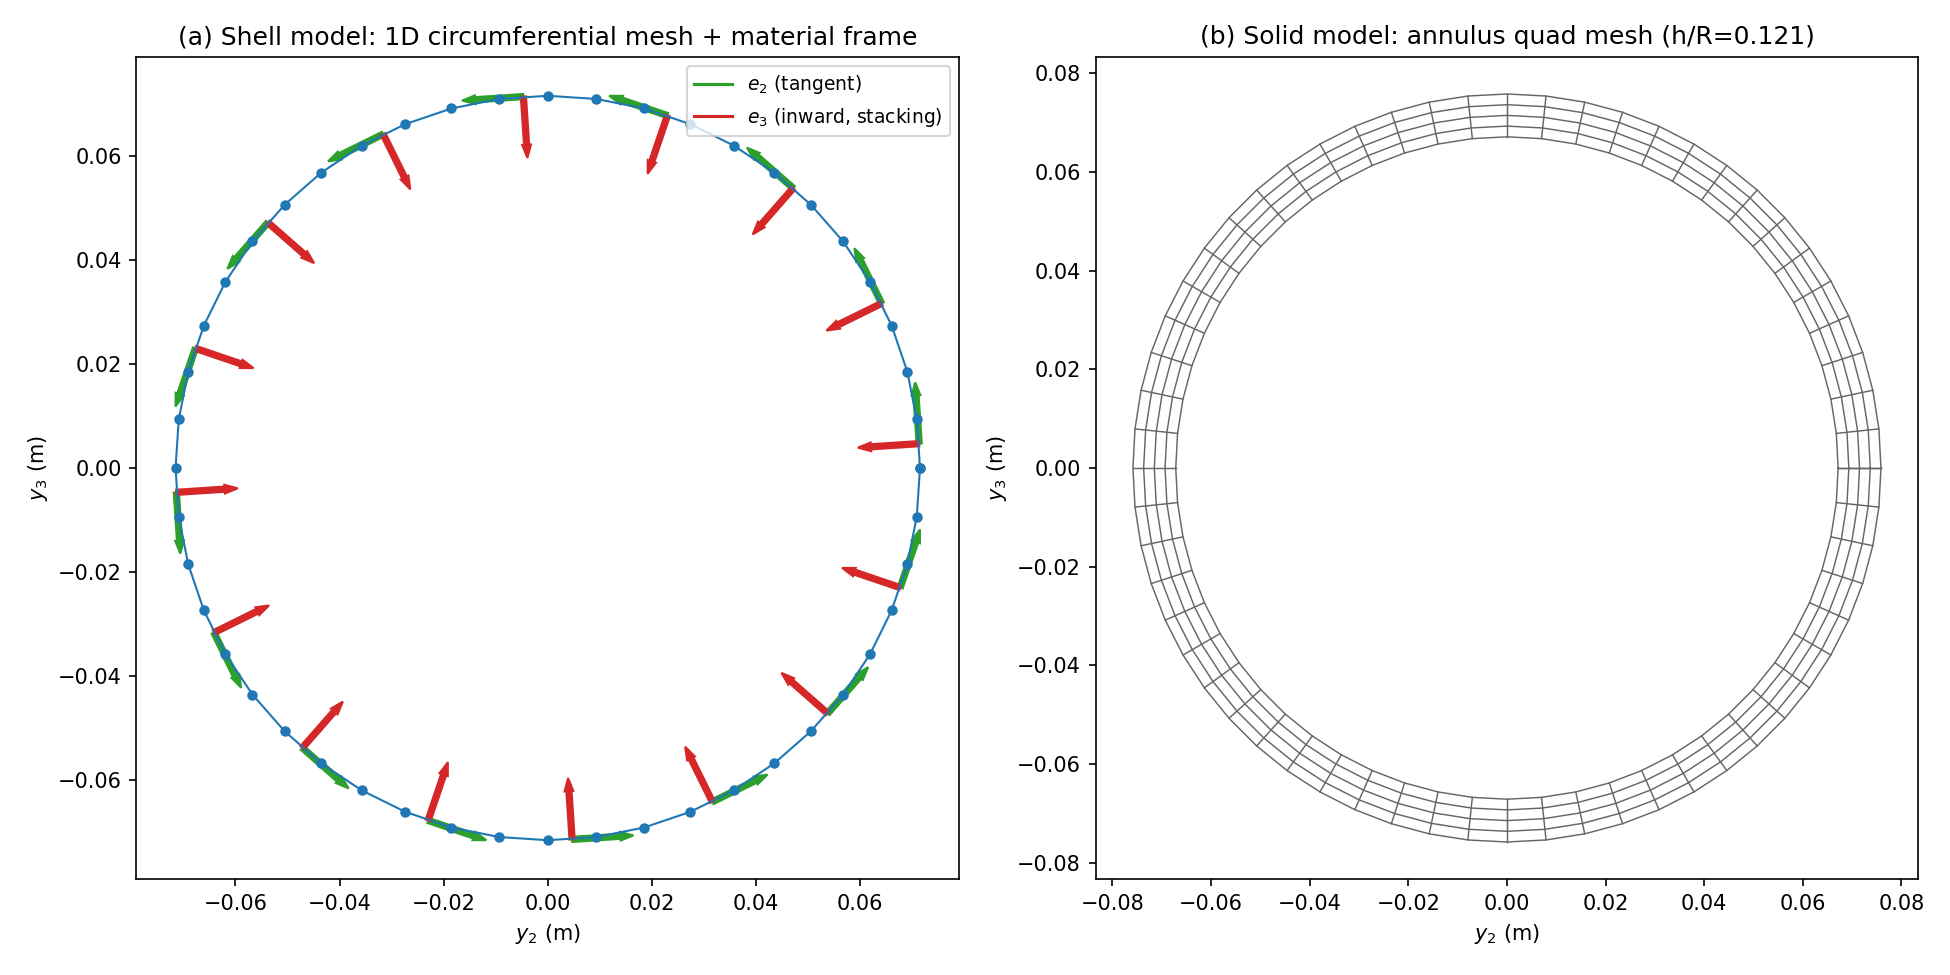
\includegraphics[width=0.92\textwidth]{fig_mesh.png}
\caption{Anisotropic tube: (a) the shell model is a 1D circumferential mesh of
the mid-surface, showing the material frame $\bm{e}_2$ (tangent) and $\bm{e}_3$
(inward, stacking direction); (b) the solid reference model is an annulus of
quadrilateral elements ($\hR=0.121$).}
\label{fig:mesh}
\end{figure}

\begin{figure}[t]\centering
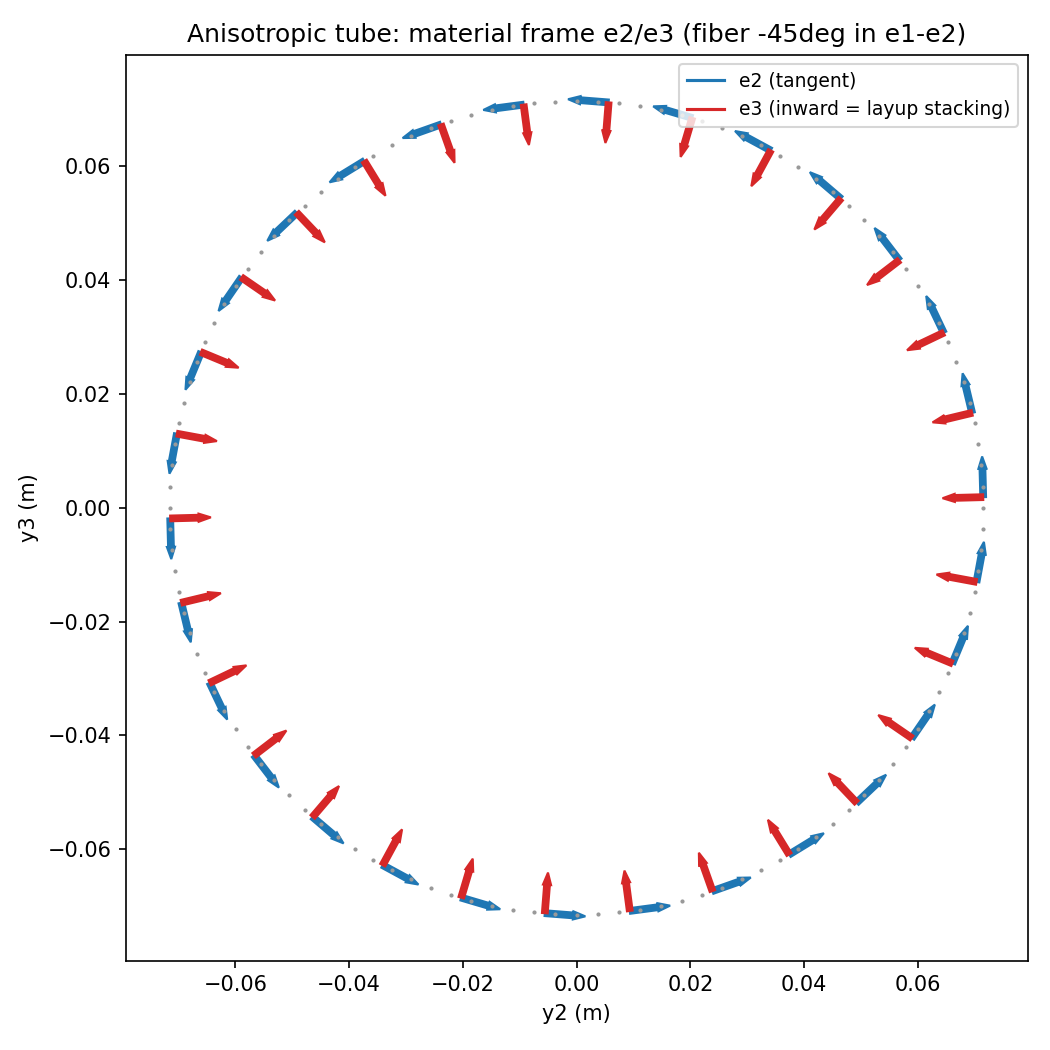
\includegraphics[width=0.62\textwidth]{fig_orientation.png}
\caption{Material frame on the shell mid-surface: $\bm{e}_2$ tangent (blue) and
$\bm{e}_3$ inward (red), consistent around the ring. The $-45^{\circ}$ fibre
lies in the $\bm{e}_1$--$\bm{e}_2$ plane. The same $\bm{e}_3$ defines both the
reference offset and the lamination stacking, an enforced consistency check.}
\label{fig:orient}
\end{figure}

\paragraph{Solid reference.} The 3D solid cross-sectional analysis discretizes
the wall annulus with first-order quadrilateral elements (Fig.~\ref{fig:mesh}b)
and applies the same MSG/VABS reduction with full 3D constitutive behaviour and
the lamina orientation baked into the element frame. It is implemented in
FEniCSx/dolfinx and serves as the high-fidelity benchmark; its $6\times6$ was
verified to be mesh-converged (invariant to within $0.01\%$ for $6$--$40$
through-thickness elements and $120$--$360$ circumferential elements).

%==============================================================
\section{Results}
%==============================================================

\subsection{Homogenization}
Table~\ref{tab:homo} compares every non-zero term of the $6\times6$ Timoshenko
stiffness for the Kirchhoff and RM shell models against the solid benchmark and
the published classical value. \textbf{All shell terms agree with the solid to
within $0.7\%$}, including the tension--twist coupling $C_{14}$ produced by the
off-axis ply and the transverse-shear stiffness $C_{22}=C_{33}$. The bending
terms $C_{55}=C_{66}$ exceed the published \emph{classical} value by $\sim15\%$;
this is not an error but the difference between the Euler--Bernoulli stiffness
(to which the published value belongs, and which our shell EB matches to
$0.2\%$) and the generalized Timoshenko stiffness, whose bending diagonal
includes the bending--shear coupling intrinsic to the $-45^{\circ}$ ply. The
solid and both shell models reproduce the \emph{same} Timoshenko value.

\begin{table}[t]\centering
\caption{Anisotropic tube ($\hR=0.121$, center reference): full Timoshenko
$6\times6$ stiffness. TW-RM and TW-Kirchhoff are the present thin-walled shell
models; ``solid'' is the 3D FE benchmark; the last column is the published
classical (EB) value where applicable. Percent errors are relative to the solid
Timoshenko benchmark.}
\label{tab:homo}
\resizebox{\textwidth}{!}{%
\begin{tabular}{lrrrrr}
\toprule
term & TW-RM & TW-Kirchhoff & solid & classical & err (RM/Kirch) \\
\midrule
$C_{11}$ (EA)            & $4.7835\!\times\!10^{7}$ & $4.7853\!\times\!10^{7}$ & $4.7843\!\times\!10^{7}$ & $4.7785\!\times\!10^{7}$ & $-0.02\%/{+}0.02\%$ \\
$C_{14}$ (ext--twist)    & $-9.3125\!\times\!10^{5}$ & $-9.2971\!\times\!10^{5}$ & $-9.3459\!\times\!10^{5}$ & $-9.3755\!\times\!10^{5}$ & $-0.36\%/{-}0.52\%$ \\
$C_{22}$ (GA$_2$)        & $1.4504\!\times\!10^{7}$ & $1.4450\!\times\!10^{7}$ & $1.4548\!\times\!10^{7}$ & --- & $-0.30\%/{-}0.67\%$ \\
$C_{33}$ (GA$_3$)        & $1.4504\!\times\!10^{7}$ & $1.4473\!\times\!10^{7}$ & $1.4548\!\times\!10^{7}$ & --- & $-0.30\%/{-}0.51\%$ \\
$C_{25}$ (shear--bend)   & $4.6958\!\times\!10^{5}$ & $4.6716\!\times\!10^{5}$ & $4.6855\!\times\!10^{5}$ & --- & $+0.22\%/{-}0.30\%$ \\
$C_{44}$ (GJ)            & $1.4822\!\times\!10^{5}$ & $1.4799\!\times\!10^{5}$ & $1.4820\!\times\!10^{5}$ & $1.4896\!\times\!10^{5}$ & $+0.01\%/{-}0.14\%$ \\
$C_{55}$ (EI$_2$)        & $1.2269\!\times\!10^{5}$ & $1.2243\!\times\!10^{5}$ & $1.2281\!\times\!10^{5}$ & $1.0710\!\times\!10^{5}$ & $-0.10\%/{-}0.31\%$ \\
$C_{66}$ (EI$_3$)        & $1.2269\!\times\!10^{5}$ & $1.2247\!\times\!10^{5}$ & $1.2281\!\times\!10^{5}$ & $1.0710\!\times\!10^{5}$ & $-0.10\%/{-}0.27\%$ \\
\bottomrule
\end{tabular}}
\end{table}

\subsection{Dehomogenization}
A representative beam load $\bm{F}=[2\!\times\!10^{4}\,\text{N},0,0,300,150,0]$
(axial force, twisting and bending moments) is applied and the 3D stress is
recovered along the through-thickness path $z_2=0,\,z_3>0$ (the top of the
tube). Figure~\ref{fig:dehom} overlays the shell and solid recoveries in the
material frame. The recovered field satisfies global equilibrium: integrating
the recovered $\sigma_{11}$ over the section returns the applied $F_1$, $M_2$
and $M_3$ to within $0.2\%$. The dominant in-plane components agree well:
$\sigma_{22}$ and $\sigma_{12}$ match the solid to within $1.5\%$, and the
$\sigma_{11}$ \emph{mean} to within $0.4\%$. The out-of-plane normal stress
$\sigma_{33}$ is negligible ($\sim\!10^{-8}$ of the in-plane level), and the
transverse-shear stresses vanish because this load carries no section shear
force. The only discernible discrepancy is the through-thickness
\emph{gradient} of $\sigma_{11}$, analyzed next.

\begin{figure}[t]\centering
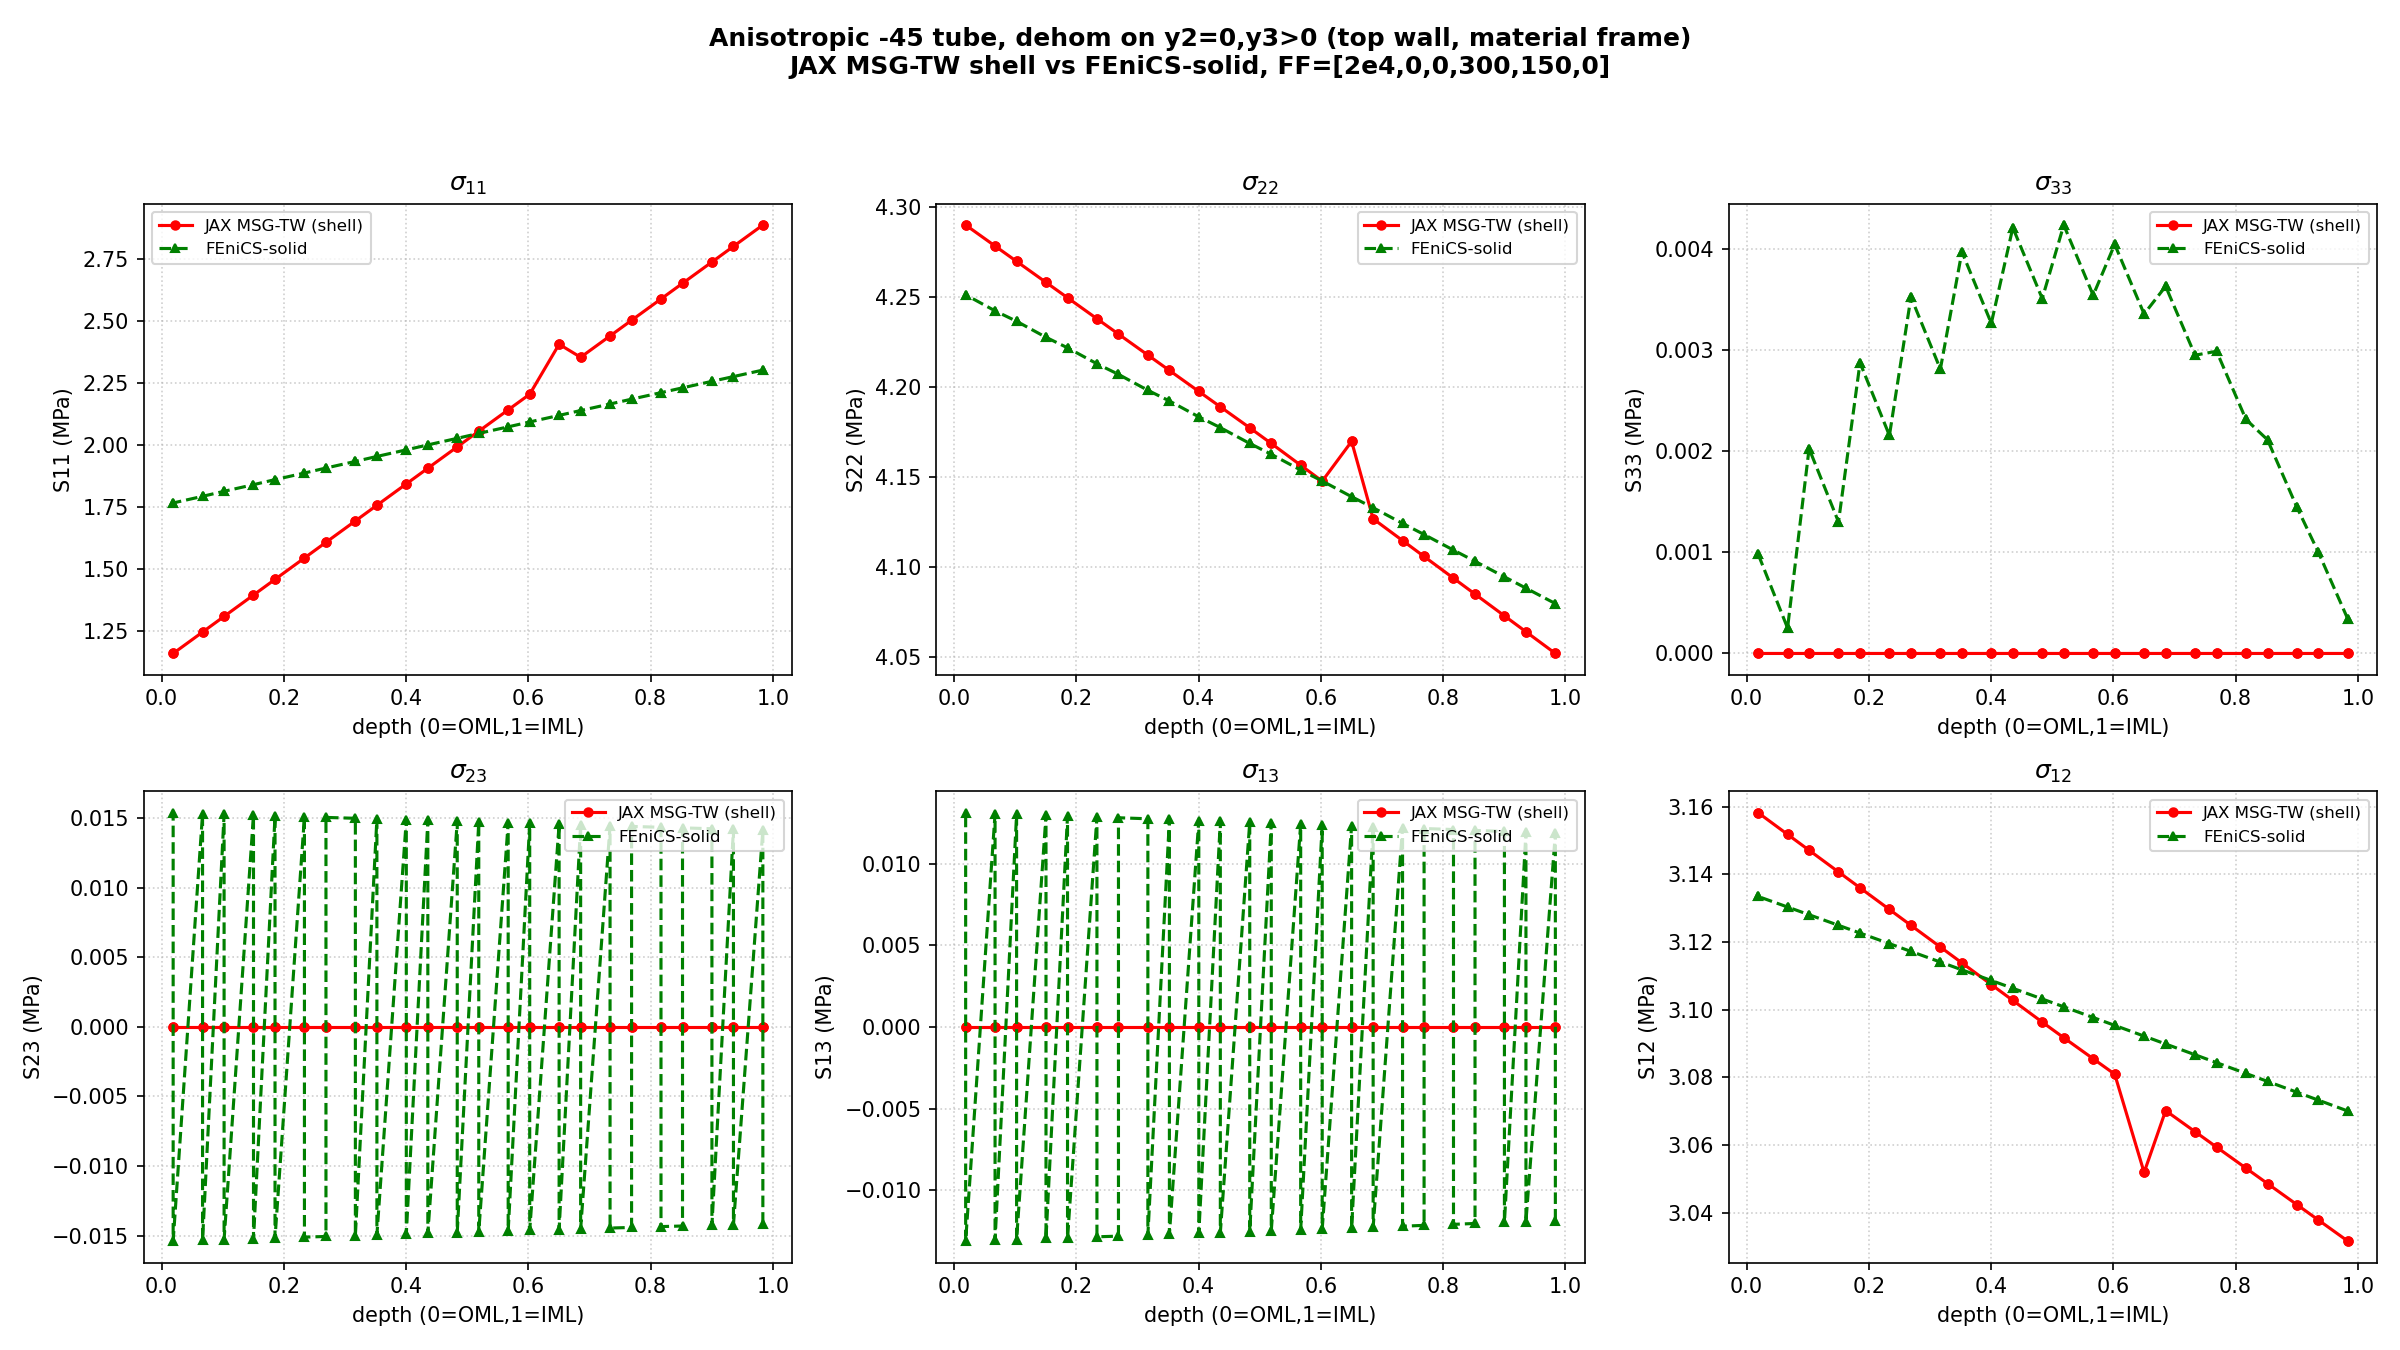
\includegraphics[width=0.96\textwidth]{fig_dehom.png}
\caption{Recovered 3D stress (material frame) on the path $z_2=0,z_3>0$ under
the representative load: shell (MSG-TW) versus solid. In-plane $\sigma_{22}$,
$\sigma_{12}$ and the $\sigma_{11}$ mean agree to within a few percent;
$\sigma_{33},\sigma_{13},\sigma_{23}\approx0$ (no section shear for this load).}
\label{fig:dehom}
\end{figure}

\subsection{Isolating the recovery from the stiffness}
To separate stiffness differences from recovery differences, both models are
driven by the \emph{same} generalized beam strain (pure extension
$\eps_{11}=1$, and pure bending $\kappa_2=1$) and the recovered $\sigma_{11}(z)$
is compared (Fig.~\ref{fig:strain}). Under pure extension the through-thickness
\emph{means} match to $2.3\%$, but the small through-thickness gradients have
opposite sign (shell $+13.5\%$, solid $-9.2\%$ of the mean): the thin-shell and
3D recoveries of the off-axis warping differ at this thickness. The gradient is
a higher-order quantity superposed on the dominant uniform field; its behaviour
with thickness is examined next.

\begin{figure}[t]\centering
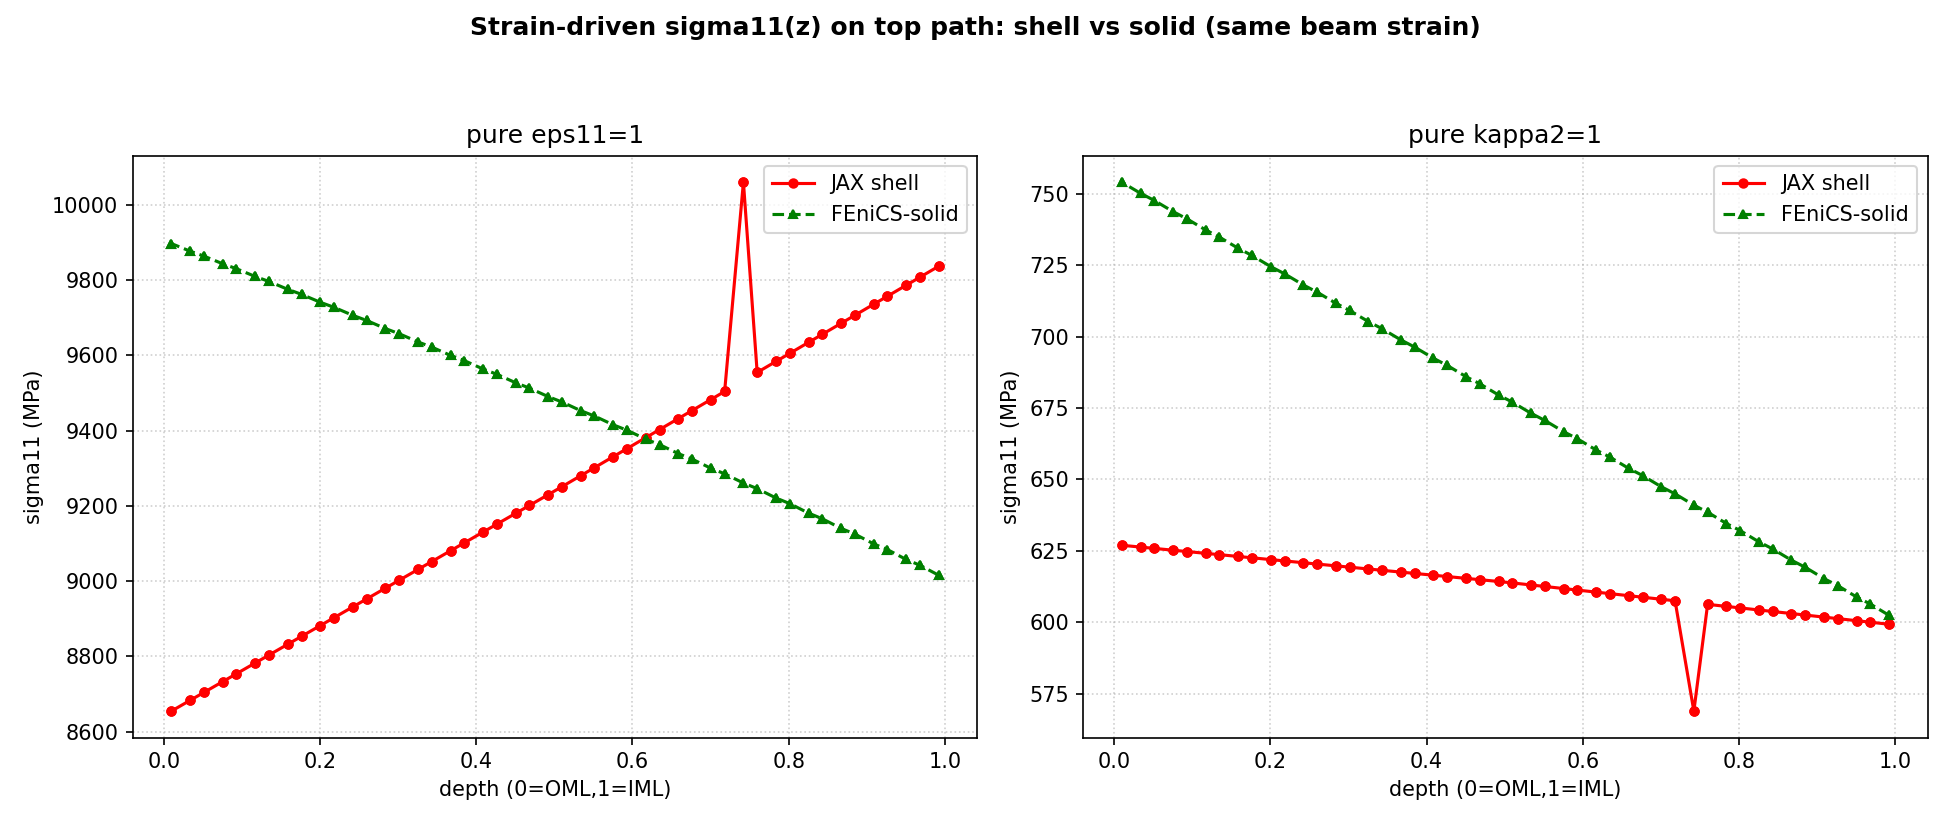
\includegraphics[width=0.92\textwidth]{fig_strain.png}
\caption{Strain-driven $\sigma_{11}(z)$ on the top path: shell versus solid
under identical beam strain (left: pure extension; right: pure bending). The
means agree; the through-thickness gradient differs, indicating a recovery (not
a stiffness) effect.}
\label{fig:strain}
\end{figure}

\subsection{Thickness convergence}
\label{sec:conv}
The wall thickness is reduced at fixed radius, $\hR=0.121\to0.015$, and the
homogenization and strain-driven recovery are repeated for both models and the
solid (Fig.~\ref{fig:conv}, Table~\ref{tab:conv}). Two clear conclusions
emerge. First, the shell and solid \emph{Timoshenko} $EI$ coincide to within
$0.15\%$ at \emph{every} thickness; the ratio of the classical (EB) to the
Timoshenko stiffness stays near $0.877$, confirming that the $\sim15\%$ offset
relative to the published value is the (thickness-independent) EB-to-Timoshenko
difference of the anisotropic section, not a discretization error. Second, the
through-thickness $\sigma_{11}$ gradient---the lone recovery discrepancy---decays
linearly with $\hR$ for both models, and the shell--solid gap halves with each
halving of $\hR$ ($22.7\%\to11.8\%\to6.8\%\to3.0\%$ of the mean). This is the
signature of an $O(\hR)$ thick-shell effect: as the wall becomes thin the shell
recovery converges to the 3D solid, as it must. The residual at the benchmark
$\hR=0.121$ is therefore the expected finite-thickness limit of classical shell
theory rather than a modelling defect; it can be reduced by a
curvature-corrected or higher-order through-thickness recovery.

\begin{table}[t]\centering
\caption{Thickness convergence. Columns: shell-to-solid Timoshenko $EI$ ratio;
through-thickness $\sigma_{11}$ gradient (\% of mean) under pure extension for
shell and solid.}
\label{tab:conv}
\small
\begin{tabular}{cccc}
\toprule
$\hR$ & shell$_{\text{Timo}}$/solid$_{\text{Timo}}$ $EI$
& shell grad/mean & solid grad/mean \\
\midrule
0.121 & 0.9985 & $+13.5\%$ & $-9.2\%$ \\
0.061 & 0.9990 & $+7.2\%$  & $-4.6\%$ \\
0.030 & 0.9999 & $+4.5\%$  & $-2.3\%$ \\
0.015 & 1.0001 & $+1.9\%$  & $-1.1\%$ \\
\bottomrule
\end{tabular}
\end{table}

\begin{figure}[t]\centering

\includegraphics[width=0.98\textwidth]{fig_convergence.png}
\caption{Thickness convergence ($\hR\to0$). Left/center: through-thickness
$\sigma_{11}$ gradient (\% of mean) under pure extension and pure bending, shell
versus solid; both tend to zero linearly in $\hR$. Right: $EI$ ratios---shell
Timoshenko/solid Timoshenko $\approx1$ at all thicknesses, while shell
EB/solid Timoshenko stays at $\approx0.877$.}
\label{fig:conv}
\end{figure}

\subsection{Out-of-plane stress: Kirchhoff versus Reissner--Mindlin}
To exercise the transverse shear, a section shear force $F_2=2\times10^{4}$~N
(whose shear flow peaks at the top of the tube) is applied and the out-of-plane
stresses are recovered on the same path (Fig.~\ref{fig:oop}). The normal stress
$\sigma_{33}$ remains negligible for both shell models and for the solid,
consistent with the plane-stress assumption. The transverse-shear stresses
$\sigma_{13},\sigma_{23}$ are \emph{identically zero} for the Kirchhoff model
(it has no transverse-shear kinematics), whereas the RM model recovers the
parabolic through-thickness profile of Eq.~\eqref{eq:shearrecov} that follows
the solid. For this thin tube the transverse-shear magnitude is small
($O(\hR)$ below the in-plane shear flow), but the qualitative distinction is
exact and becomes important for shear-dominated or thicker sections (e.g.\ shear
webs), where the RM model captures stresses the Kirchhoff model cannot.

\begin{figure}[t]\centering
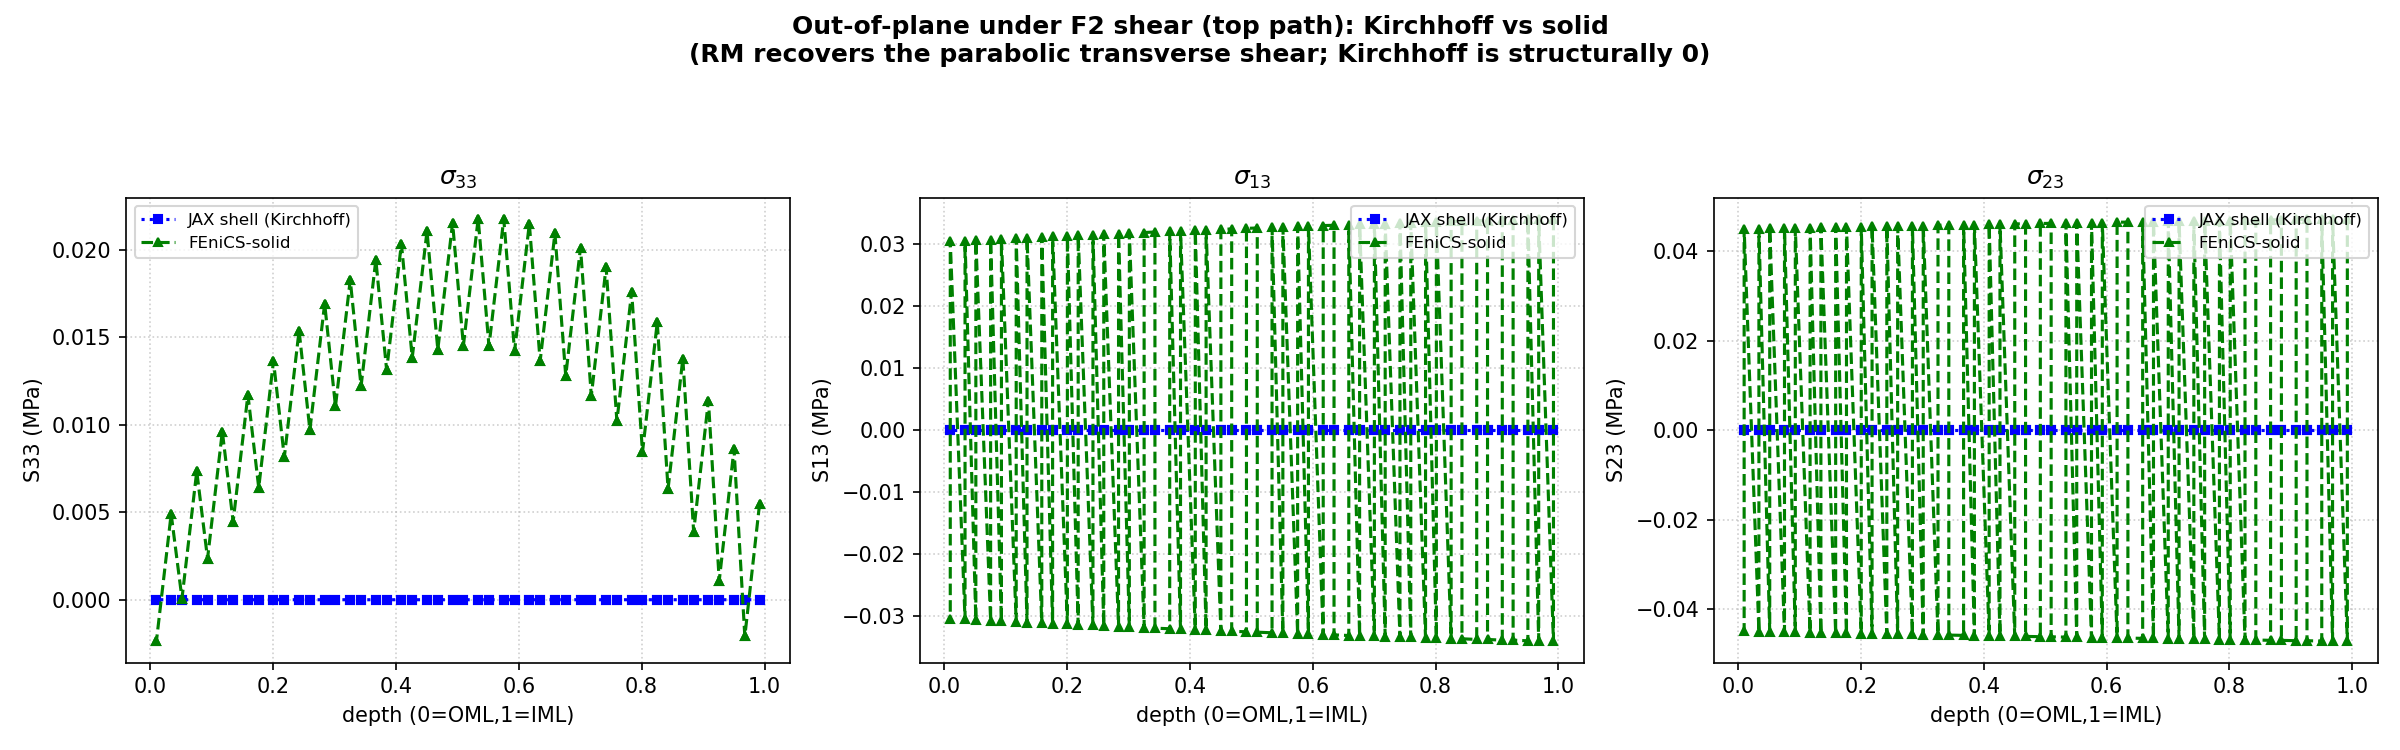
\includegraphics[width=0.96\textwidth]{fig_oop.png}
\caption{Out-of-plane stress under a section shear force $F_2$: $\sigma_{33}$,
$\sigma_{13}$, $\sigma_{23}$ on the top path. Kirchhoff returns zero transverse
shear by construction; the RM recovery follows the solid.}
\label{fig:oop}
\end{figure}

%==============================================================
\section{Application to a wind-turbine blade cross-section}
\label{sec:blade}
%==============================================================
To demonstrate the method on a realistic multi-material section, we analyze
station~15 of a utility-scale wind-turbine blade (the \texttt{bar\_urc} model).
The cross-section (Fig.~\ref{fig:st15sec}a) is a deep, multi-region laminate
comprising unidirectional spar caps, two shear webs, foam-cored sandwich panels,
and leading-/trailing-edge reinforcements. The high-fidelity reference is VABS,
which performs a two-dimensional \emph{solid} finite-element cross-sectional
analysis; we use its Timoshenko stiffness (\texttt{.K}) and recovered stress
(\texttt{.SM}) outputs.

\subsection{Homogenization}
Table~\ref{tab:st15} compares the principal Timoshenko stiffnesses of the
present shell models against VABS. The axial, shear and flapwise-bending
stiffnesses ($EA$, $GA_2$, $GA_3$, $EI_2$) agree to within $\sim$2--10\%, and
the extension--bending coupling $C_{16}$ to within 9\%; the relative norm over
all twelve non-zero terms is $5.6\%$ for both shell models. Both models capture
the torsional stiffness to within $\sim$5\% ($GJ$: $-4.9\%$ for RM, $-3.6\%$ for
Kirchhoff); for this closed, membrane-dominated section the two are comparable,
as expected (the RM/Kirchhoff torsion split is an open-section effect). The chordwise
bending stiffness $EI_3$ is high by $\sim$14\%---the same thick-section
signature quantified for the tube in Section~\ref{sec:conv}, here because the
deep root section is locally thick relative to its radius of curvature.

\begin{table}[t]\centering
\caption{Station-15 principal Timoshenko stiffnesses: present shell models
versus VABS (2D solid FE). The relative norm over all twelve non-zero
$6\times6$ terms is $5.6\%$ for both models.}
\label{tab:st15}
\resizebox{\textwidth}{!}{%
\begin{tabular}{lrrrr}
\toprule
term & TW-RM & TW-Kirchhoff & VABS & err (RM/Kirch)\\
\midrule
$C_{11}$ (EA)        & $1.3326\!\times\!10^{10}$ & $1.3326\!\times\!10^{10}$ & $1.3083\!\times\!10^{10}$ & $+1.9\%/{+}1.9\%$\\
$C_{16}$ (ext--bend) & $-3.241\!\times\!10^{9}$  & $-3.242\!\times\!10^{9}$  & $-3.571\!\times\!10^{9}$  & $-9.2\%/{-}9.2\%$\\
$C_{22}$ (GA$_2$)    & $4.409\!\times\!10^{8}$   & $4.462\!\times\!10^{8}$   & $4.580\!\times\!10^{8}$   & $-3.7\%/{-}2.6\%$\\
$C_{33}$ (GA$_3$)    & $9.507\!\times\!10^{7}$   & $9.627\!\times\!10^{7}$   & $1.055\!\times\!10^{8}$   & $-9.9\%/{-}8.8\%$\\
$C_{44}$ (GJ)        & $1.484\!\times\!10^{8}$   & $1.504\!\times\!10^{8}$   & $1.560\!\times\!10^{8}$   & $-4.9\%/{-}3.6\%$\\
$C_{55}$ (EI$_2$)    & $1.6715\!\times\!10^{9}$  & $1.6716\!\times\!10^{9}$  & $1.6630\!\times\!10^{9}$  & $+0.5\%/{+}0.5\%$\\
$C_{66}$ (EI$_3$)    & $5.809\!\times\!10^{9}$   & $5.809\!\times\!10^{9}$   & $5.107\!\times\!10^{9}$   & $+13.8\%/{+}13.7\%$\\
\bottomrule
\end{tabular}}
\end{table}

\begin{figure}[t]\centering
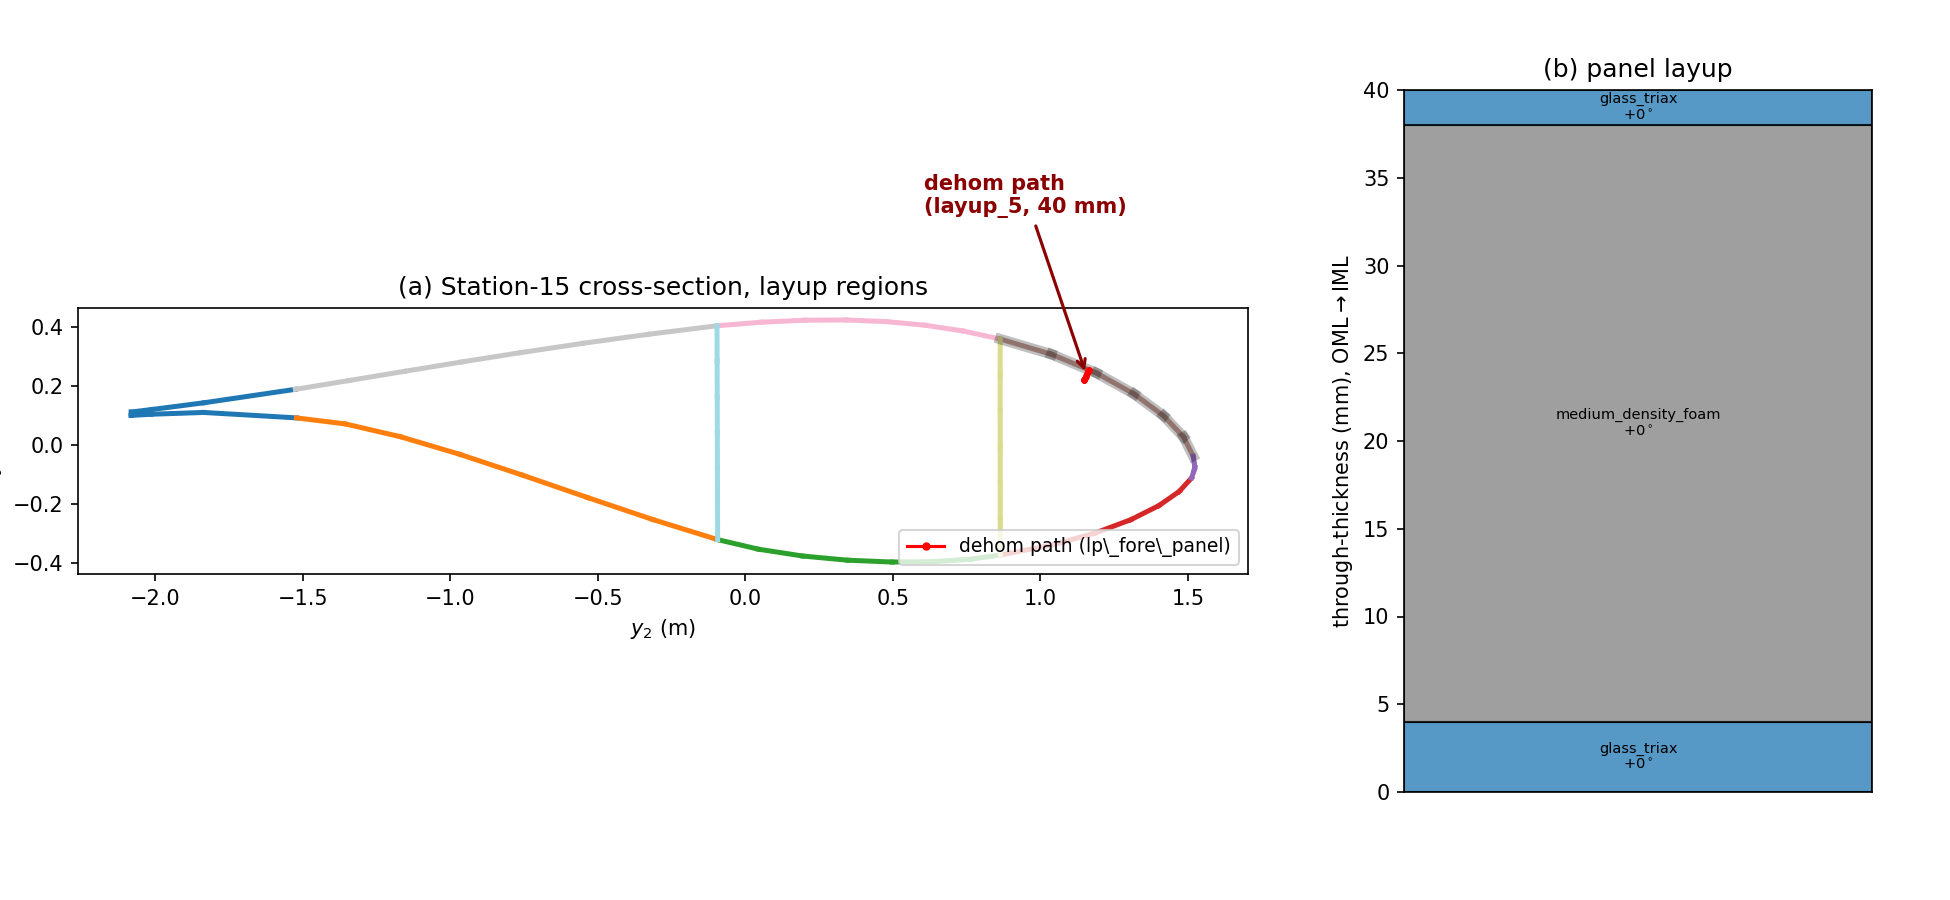
\includegraphics[width=0.98\textwidth]{fig_st15_section.png}
\caption{(a) Station-15 cross-section with layup regions (spar caps, two shear
webs, sandwich panels, LE/TE reinforcements); the highlighted line is the
through-thickness dehomogenization path in the low-pressure fore sandwich panel.
(b) The panel layup: thin glass-triax structural skins (4 and 2~mm) bonding a
34~mm foam core.}
\label{fig:st15sec}
\end{figure}

\subsection{Dehomogenization on a thin sandwich panel}
Guided by the thickness study (Section~\ref{sec:conv}), which shows the shell
recovery converging to the solid as the wall thins, we recover the 3D stress on
a through-thickness path in the low-pressure fore sandwich panel
(Fig.~\ref{fig:st15sec}). Although the panel is 40~mm overall, its load-carrying
laminate is two \emph{thin} glass skins (4 and 2~mm) separated by a soft foam
core---the archetypal thin-walled-shell region. Under a representative
blade-section load, the recovered material-frame stress
(Fig.~\ref{fig:st15deh}) matches VABS closely: the dominant axial stress
$\sigma_{11}$, carried almost entirely by the skins, agrees to within $1.4\%$
($21.7$ versus $21.4$~MPa peak), while the foam core is correctly near
stress-free. The in-plane shear $\sigma_{12}$ tracks VABS to within its small
magnitude, and the out-of-plane components $\sigma_{33},\sigma_{13},\sigma_{23}$
are negligible, as expected away from junctions. The Kirchhoff and RM in-plane
recoveries coincide (they share the membrane--bending response); the RM model
additionally returns the small parabolic transverse-shear profile that Kirchhoff
sets to zero. This confirms, on a realistic blade laminate, that in the
thin-walled regions for which the model is intended the shell dehomogenization
reproduces the solid (VABS) stress field.

\begin{figure}[t]\centering
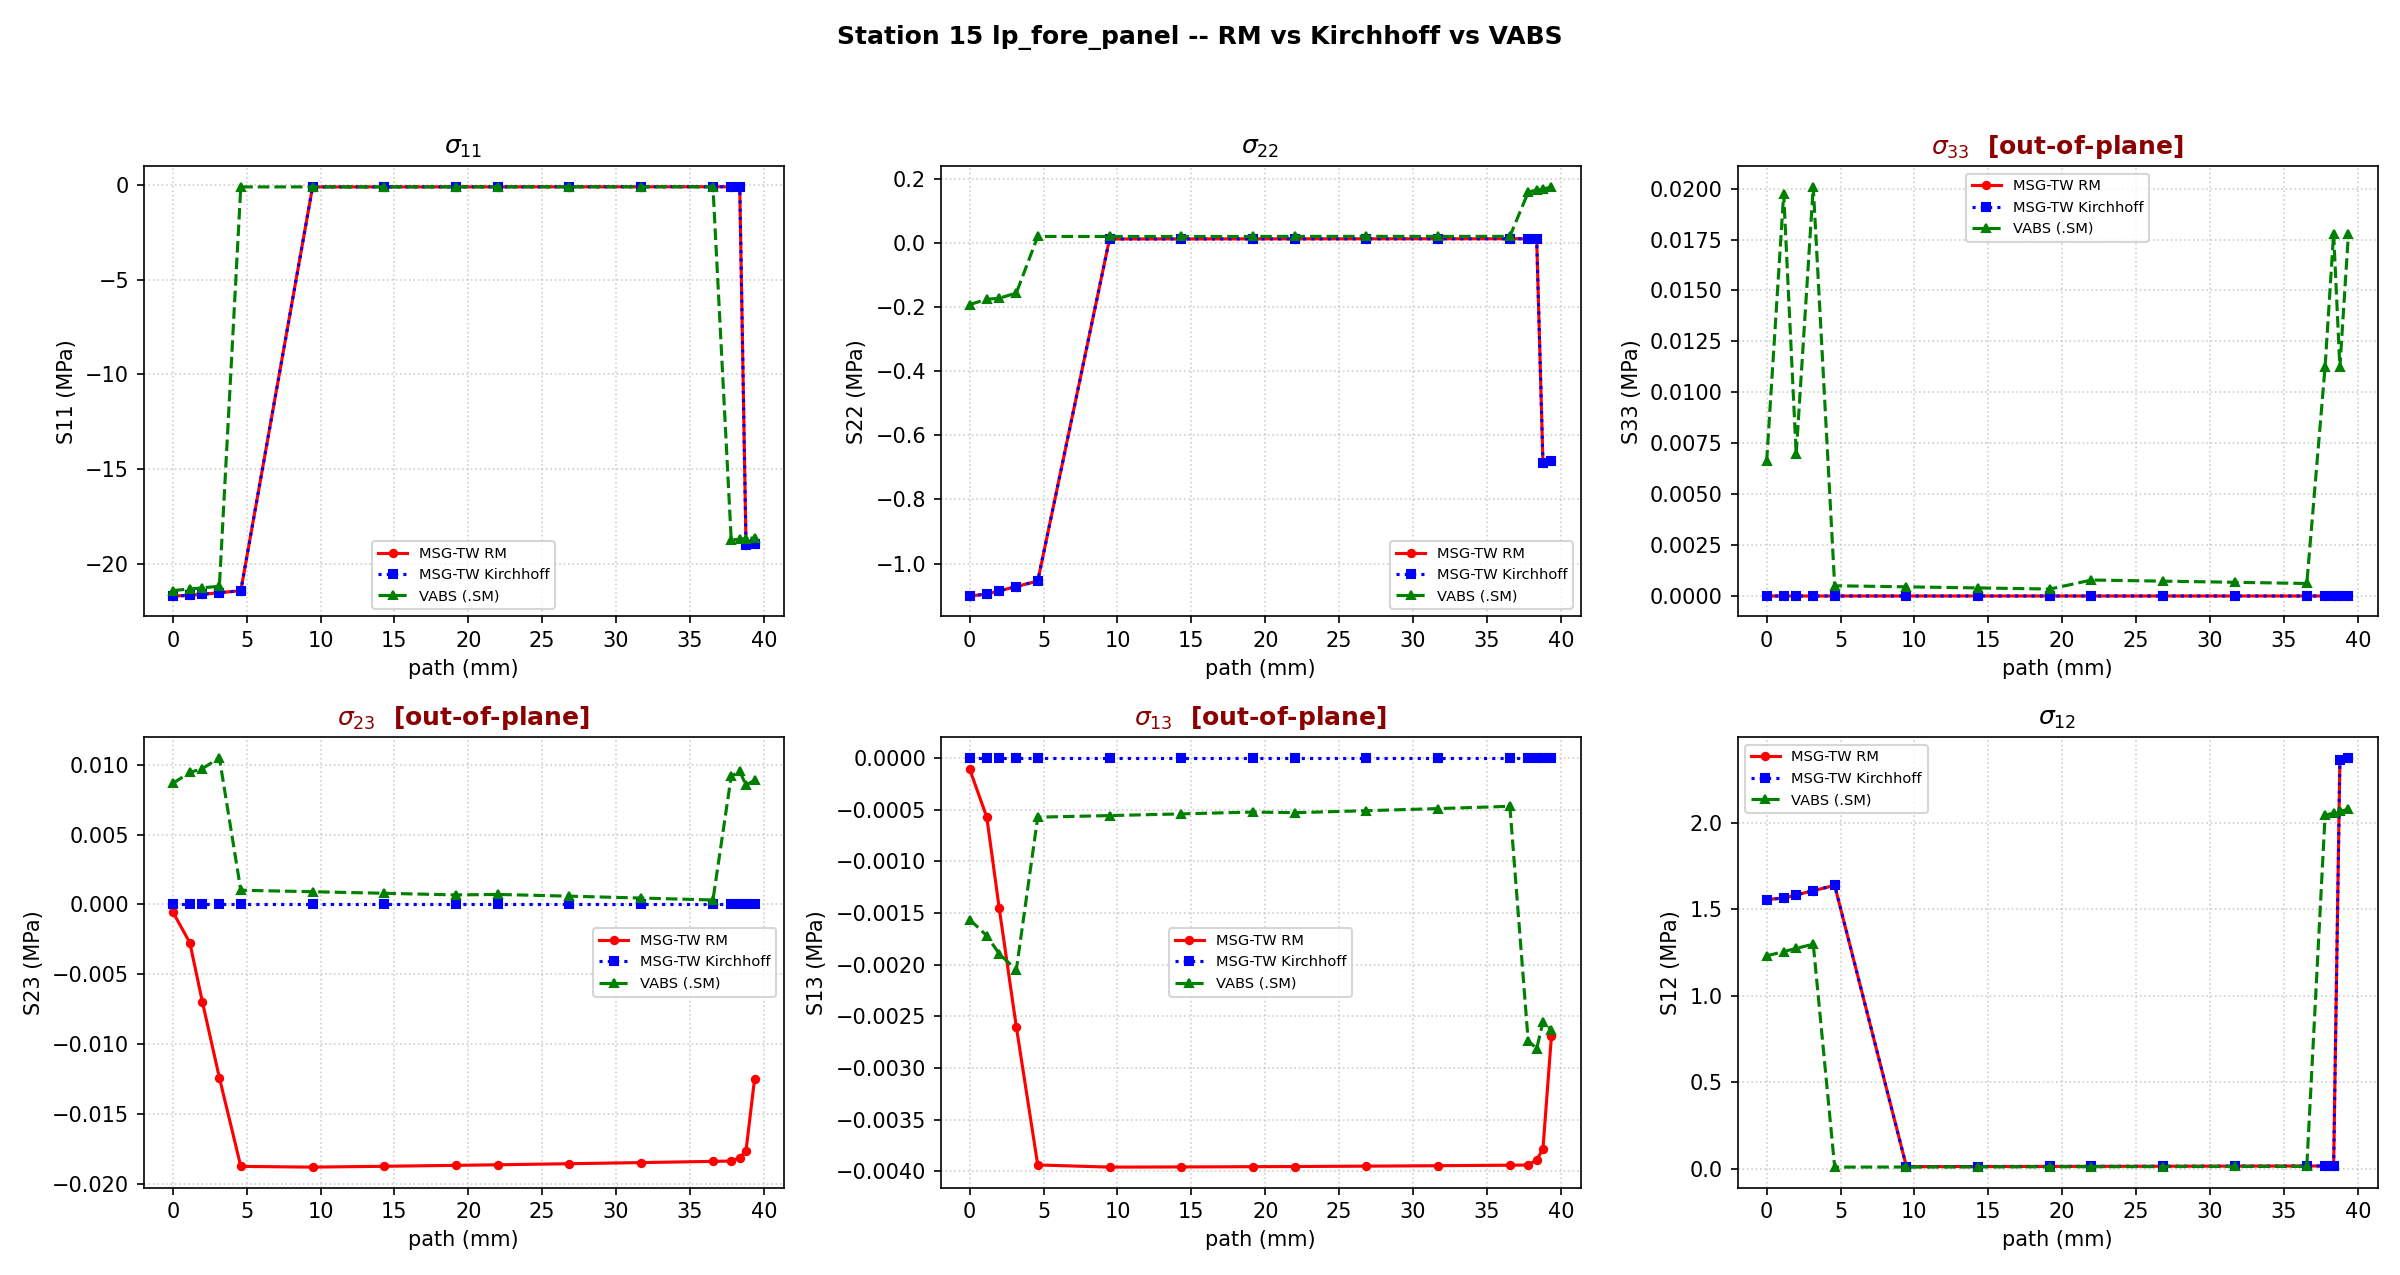
\includegraphics[width=0.98\textwidth]{fig_st15_dehom.png}
\caption{Station-15 recovered 3D stress (material frame) through the thickness
of the low-pressure fore sandwich panel: present shell models (TW-RM,
TW-Kirchhoff) versus VABS. The axial stress $\sigma_{11}$ concentrates in the
thin skins and matches VABS within $1.4\%$; the foam core is near stress-free;
out-of-plane components are negligible.}
\label{fig:st15deh}
\end{figure}

\subsection{Independent solid cross-check at a neighbouring station}
\label{sec:st13}
The station-15 comparison used VABS as the reference. As an independent check
with the present FEniCS 2D-solid analysis, we benchmark a neighbouring station
for which a solid mesh is available. The supplied solid mesh, although labelled
``12'', is located at $x_1=44.83\,\text{m}=\tfrac{13}{29}\times100\,\text{m}$,
i.e.\ \emph{station 13}; matching it against the candidate shell sections
confirms this---the $6\times6$ relative norm is minimized at station 13 ($5.5\%$),
versus $13.9\%$, $19.3\%$ and $27.9\%$ for stations 12, 11 and 10 (the axial
stiffness, being reference-independent, pins the station). Comparing the
mislabelled station gave a spurious $\sim$30\% bending error that is, in fact, a
one-station offset.

Table~\ref{tab:st13} compares the shell $6\times6$ (centroid reference) for
\texttt{1Dshell\_13} against the FEniCS-solid; the agreement matches the st15
quality---principal stiffnesses within $1.5$--$8.7\%$ and a relative norm of
$5.5\%$ for both shell models. Under a representative bending--torsion load
$\bm{F}=[2,0,0,3,8,5]\times10^5$, the 3D stress recovered on a through-thickness
path in the fore sandwich panel (Fig.~\ref{fig:st13deh}) matches the solid: the
axial stress $\sigma_{11}$ (carried by the skins) to $+4.0\%$ and the torsional
shear flow $\sigma_{12}$ to $+10.8\%$, with the foam core near stress-free. The
small transverse shear $\sigma_{23}$ ($0.1$~MPa in the solid) is the component
the Kirchhoff recovery sets to zero and the RM model supplies.

\begin{table}[t]\centering
\caption{Station-13 principal Timoshenko stiffnesses: present shell models vs
the FEniCS 2D-solid. Relative norm over the non-zero $6\times6$ terms: $5.5\%$
(both models).}
\label{tab:st13}
\resizebox{\textwidth}{!}{%
\begin{tabular}{lrrrr}
\toprule
term & TW-RM & TW-Kirchhoff & solid & err (RM/Kirch)\\
\midrule
$C_{11}$ (EA)        & $1.4094\!\times\!10^{10}$ & $1.4095\!\times\!10^{10}$ & $1.4315\!\times\!10^{10}$ & $-1.5\%/{-}1.5\%$\\
$C_{16}$ (ext--bend) & $-3.829\!\times\!10^{9}$  & $-3.830\!\times\!10^{9}$  & $-4.371\!\times\!10^{9}$  & $-12.4\%/{-}12.4\%$\\
$C_{22}$ (GA$_2$)    & $5.234\!\times\!10^{8}$   & $5.272\!\times\!10^{8}$   & $5.441\!\times\!10^{8}$   & $-3.8\%/{-}3.1\%$\\
$C_{33}$ (GA$_3$)    & $1.300\!\times\!10^{8}$   & $1.313\!\times\!10^{8}$   & $1.282\!\times\!10^{8}$   & $+1.5\%/{+}2.4\%$\\
$C_{44}$ (GJ)        & $2.616\!\times\!10^{8}$   & $2.640\!\times\!10^{8}$   & $2.425\!\times\!10^{8}$   & $+7.9\%/{+}8.9\%$\\
$C_{55}$ (EI$_2$)    & $2.620\!\times\!10^{9}$   & $2.621\!\times\!10^{9}$   & $2.443\!\times\!10^{9}$   & $+7.2\%/{+}7.3\%$\\
$C_{66}$ (EI$_3$)    & $7.810\!\times\!10^{9}$   & $7.811\!\times\!10^{9}$   & $7.185\!\times\!10^{9}$   & $+8.7\%/{+}8.7\%$\\
\bottomrule
\end{tabular}}
\end{table}

\begin{figure}[t]\centering
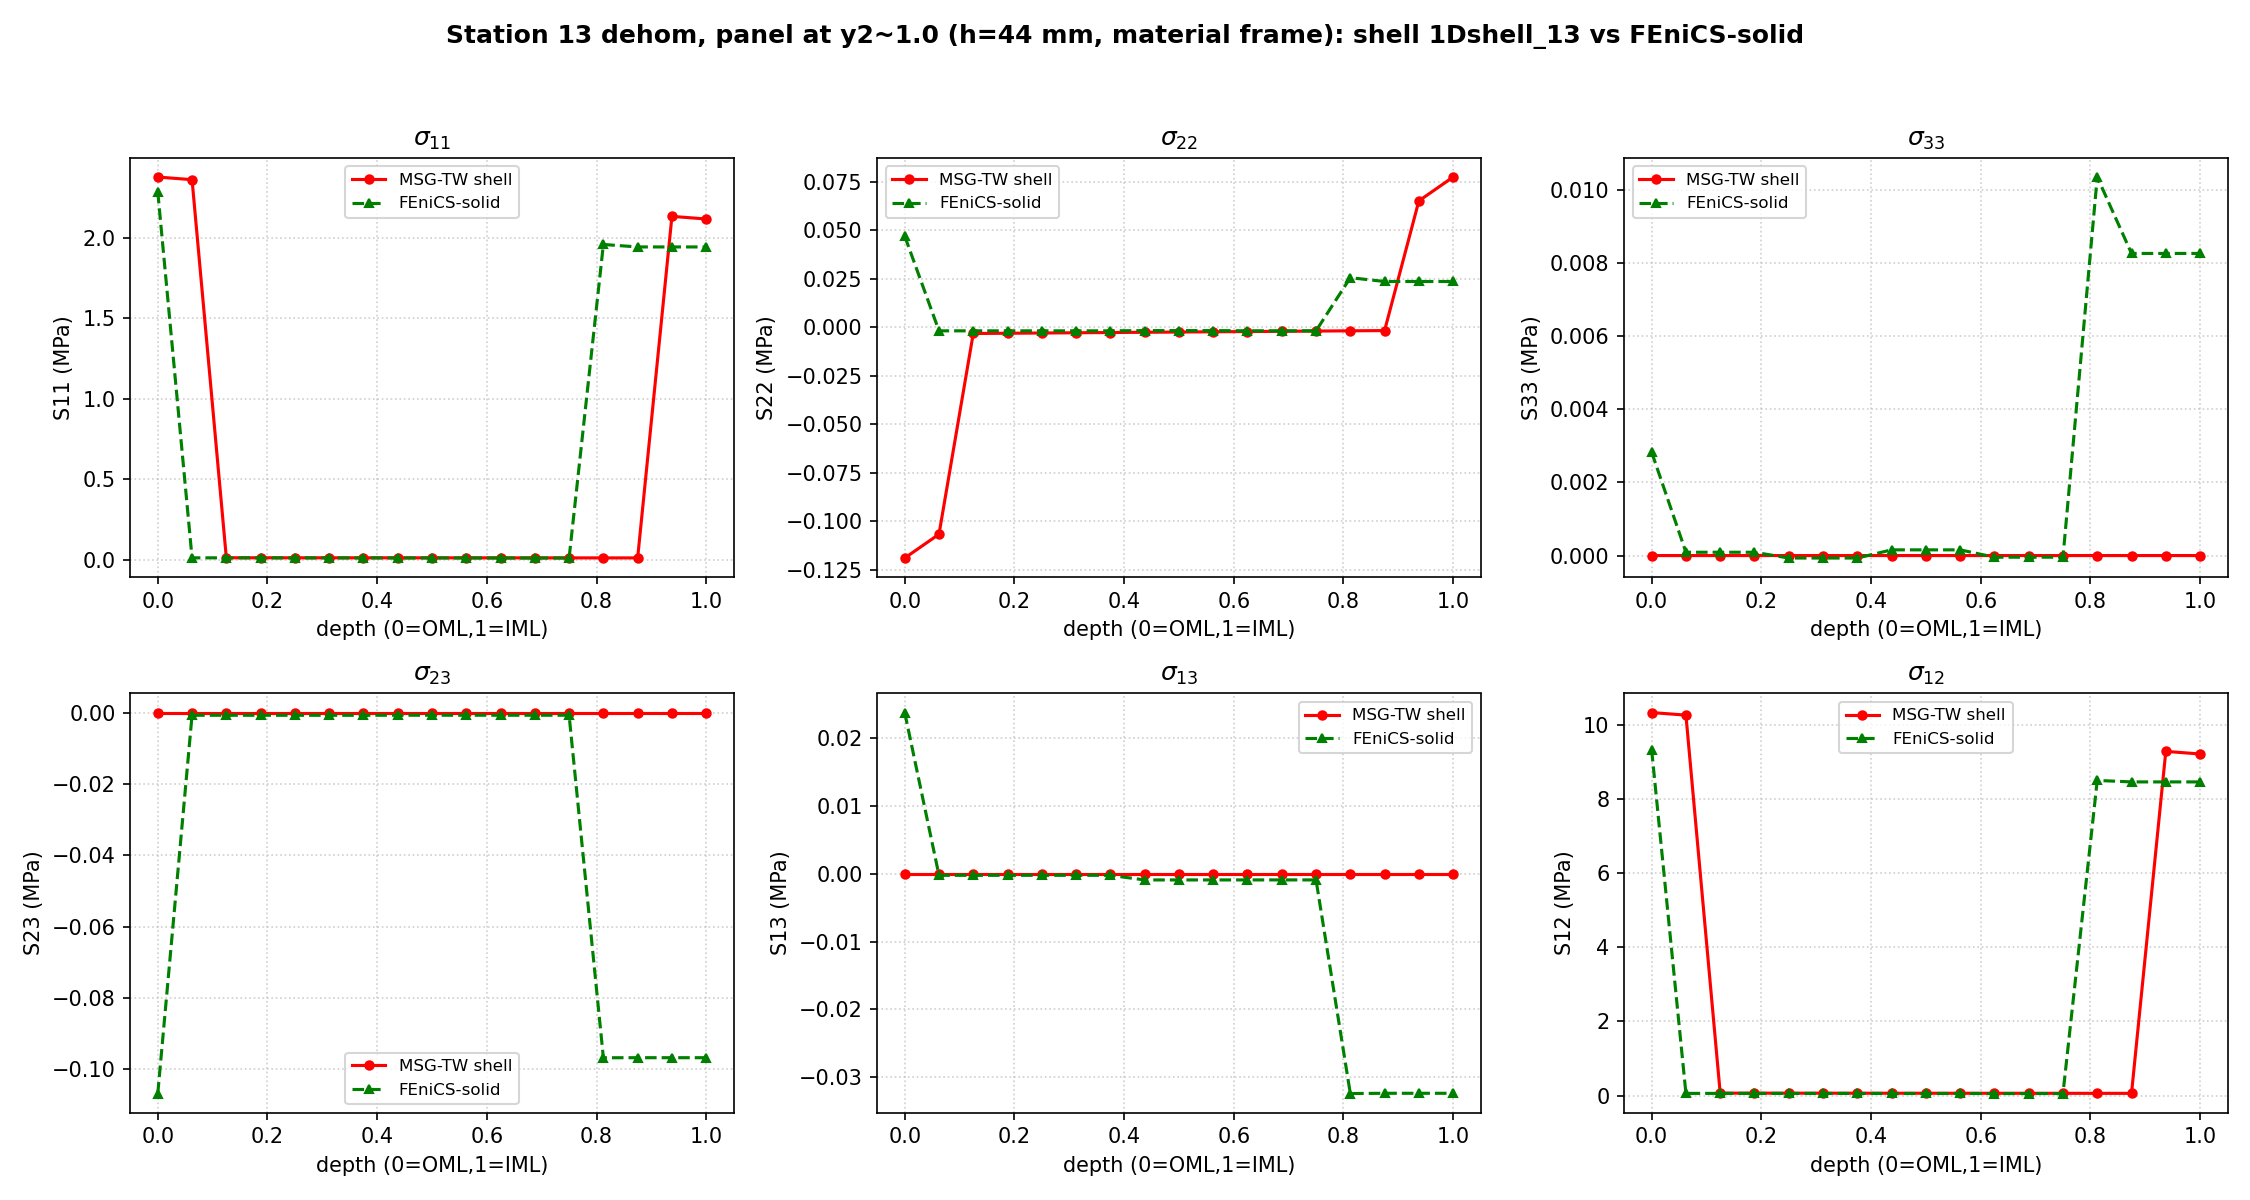
\includegraphics[width=0.96\textwidth]{fig_st13_dehom.png}
\caption{Station-13 recovered 3D stress (material frame) through the fore
sandwich panel (44~mm), shell \texttt{1Dshell\_13} vs FEniCS-solid, under a
bending--torsion load. The axial stress $\sigma_{11}$ (skins) matches to $+4\%$
and the torsional shear $\sigma_{12}$ to $+11\%$; the foam core is near
stress-free. The small $\sigma_{23}$ in the solid is the transverse shear the
Kirchhoff recovery omits.}
\label{fig:st13deh}
\end{figure}

%==============================================================
\section{Discussion}
%==============================================================
The results establish that a 1D thin-walled MSG shell analysis reproduces a 3D
solid cross-sectional analysis to engineering accuracy for the anisotropic
benchmark. Three points merit emphasis. (1) The apparent $\sim15\%$ disagreement
of the bending stiffness with the published value is a comparison artefact: the
published number is the classical (EB) stiffness, whereas the relevant quantity
for a deformable beam is the generalized Timoshenko stiffness; shell and solid
agree on the latter to $0.15\%$ at all thicknesses, and the EB-to-Timoshenko
gap is an intrinsic, thickness-independent property of the off-axis section.
(2) The dominant recovered stresses ($\sigma_{22}$, $\sigma_{12}$, the
$\sigma_{11}$ mean) match the solid to within a few percent; the only residual
is the through-thickness $\sigma_{11}$ gradient, which the thickness study
identifies unambiguously as an $O(\hR)$ thick-shell recovery effect that
vanishes in the thin limit. For thick walls ($\hR\gtrsim0.1$) this gradient
should be recovered with a curvature-corrected plate metric or a higher-order
through-thickness theory. (3) Retaining transverse shear (RM) is essential when
the recovered transverse-shear stress is of interest---a quantity that the
Kirchhoff model omits identically---at negligible additional cost
($C^{0}$ Lagrange versus $C^{1}$ Hermite), provided shear locking is controlled
by selective reduced integration.

The thin-walled shell analysis reduces the cross-section to a 1D problem and is
implemented without a finite-element library or MPI, making it attractive for
design-loop and optimization use where many cross-sections must be evaluated;
the 3D solid analysis remains the reference for thick or geometrically complex
sections.

%==============================================================
\section{Conclusions}
%==============================================================
A thin-walled cross-sectional analysis for composite beams was formulated on a
1D shell structure genome with two interchangeable wall kinematics (Kirchhoff
$C^{1}$ and Reissner--Mindlin $C^{0}$), an $8\times8$ plate constitutive law
combining CLT with an FSDT transverse-shear block, asymptotic
Euler--Bernoulli/Timoshenko stiffness, and a consistent 3D stress recovery.
Validated against a 3D solid analysis on an anisotropic $-45^{\circ}$ tube:
\begin{itemize}
\item every Timoshenko $6\times6$ term matches the solid to within $0.7\%$ at
$\hR=0.121$, including the tension--twist coupling;
\item the recovered in-plane $\sigma_{22},\sigma_{12}$ and the $\sigma_{11}$
mean match to within $1.5\%$, with global equilibrium satisfied to $0.2\%$;
\item a thickness sweep shows the shell and solid Timoshenko stiffnesses
coincide to $<0.15\%$ at all $\hR$, while the sole recovery discrepancy (the
$\sigma_{11}$ gradient) decays linearly with $\hR$, confirming an $O(\hR)$
thick-shell limit;
\item the RM model recovers the transverse-shear stresses that the Kirchhoff
model omits by construction;
\item on realistic wind-turbine blade stations (multi-region laminates with
spar caps, shear webs and sandwich panels) the homogenized $6\times6$ matches
the solid references to a $5.5$--$5.6\%$ relative norm---against VABS at
station 15 and, independently, against the present FEniCS 2D-solid at
station 13---and the recovered stress in a thin sandwich panel agrees to within
$1.4\%$ (st15, vs VABS) and $4$--$11\%$ (st13, vs FEniCS-solid).
\end{itemize}
Future work will incorporate the wall-curvature metric in the through-thickness
recovery to extend the accuracy of the $\sigma_{11}$ gradient into the
thick-wall regime, and will apply the method to additional multi-cell airfoil
sections and junction regions.

%==============================================================
\section*{Data and code availability}
The cross-sectional analysis and the scripts that generate every figure and
table are available from the author on reasonable request.

\section*{Declaration of competing interest}
The author declares no competing interests.

%==============================================================
\begin{thebibliography}{20}

\bibitem{hodges2006} D.~H. Hodges,
\emph{Nonlinear Composite Beam Theory}, AIAA, Reston, VA, 2006.

\bibitem{yu2002} W.~Yu, D.~H. Hodges, V.~V. Volovoi, C.~E.~S. Cesnik,
On Timoshenko-like modeling of initially curved and twisted composite beams,
Int. J. Solids Struct. 39 (19) (2002) 5101--5121.

\bibitem{cesnik1997} C.~E.~S. Cesnik, D.~H. Hodges,
VABS: a new concept for composite rotor blade cross-sectional modeling,
J. Am. Helicopter Soc. 42 (1) (1997) 27--38.

\bibitem{yu2012vabs} W.~Yu, D.~H. Hodges, J.~C. Ho,
Variational asymptotic beam sectional analysis -- an updated version,
Int. J. Eng. Sci. 59 (2012) 40--64.

\bibitem{yu2016msg} W.~Yu,
A unified theory for constitutive modeling of composites,
J. Mech. Mater. Struct. 11 (4) (2016) 379--411.

\bibitem{liu2017msg} X.~Liu, W.~Yu,
A novel approach to analyze beam-like composite structures using mechanics of
structure genome, Adv. Eng. Softw. 100 (2017) 238--251.

\bibitem{reissner1945} E.~Reissner,
The effect of transverse shear deformation on the bending of elastic plates,
J. Appl. Mech. 12 (2) (1945) A69--A77.

\bibitem{mindlin1951} R.~D. Mindlin,
Influence of rotatory inertia and shear on flexural motions of isotropic,
elastic plates, J. Appl. Mech. 18 (1) (1951) 31--38.

\bibitem{jones1999} R.~M. Jones,
\emph{Mechanics of Composite Materials}, 2nd ed., Taylor \& Francis, 1999.

\bibitem{giavotto1983} V.~Giavotto, M.~Borri, P.~Mantegazza, G.~Ghiringhelli,
Anisotropic beam theory and applications, Comput. Struct. 16 (1--4) (1983)
403--413.

\bibitem{hodges1990} D.~H. Hodges,
A review of composite rotor blade modeling,
AIAA J. 28 (3) (1990) 561--565.

\bibitem{berdichevsky1979} V.~L. Berdichevsky,
Variational-asymptotic method of constructing a theory of shells,
J. Appl. Math. Mech. 43 (4) (1979) 711--736.

\bibitem{liu2019msg} X.~Liu, W.~Yu, A.~R. Gaonkar,
Two-step homogenization of textile composites using mechanics of structure
genome, Compos. Struct. 171 (2017) 252--262.

\bibitem{chen2010} H.~Chen, W.~Yu, M.~Capellaro,
A critical assessment of computer tools for calculating composite wind turbine
blade properties, Wind Energy 13 (6) (2010) 497--516.

\bibitem{alnaes2015} M.~Aln\ae s et al.,
The FEniCS Project Version 1.5, Arch. Numer. Softw. 3 (100) (2015) 9--23.

\end{thebibliography}

\end{document}
